\chap{A Smartphone Sensor-based Contextual Reminder Delivery Framework} \label{chapter: treatment-framework}

\setlength{\epigraphwidth}{.50\textwidth}
\begin{epigraphs}
\qitem{Memory is a mental stabilizer and without it the mind becomes chaotic and unstructured, allowing 1999 and 1940 to merge.} %Quote
{--- \textsc{Thomas DeBaggio} \\ \textit{Losing My Mind: An Intimate Look at Life with Alzheimer's}}
\end{epigraphs}

This Chapter details the design of a context-aware reminder delivery framework, aimed to improve reminder adherence for PwD. The Chapter begins by detailing the development of an assistive reminder app, equipped with bespoke usage and sensor monitoring tools. The app is tested and evaluated by a group of healthy adults, bringing note to areas for improvement. The refined app is then deployed to 30 PwD as an intervention tool for 12 months. Post-study analysis of the sensor and usage data is performed, culminating in the testing and evaluation of various classification models for the system.

\section{Introduction}
As mentioned in Chapter \ref{chapter: lit-review}, Section \ref{section: treatment-stateoftheart}, the current application of technology within dementia treatment aims to improve a PwD's health outcomes by supporting their independence and improving the quality, and timeliness, of their care. A vast majority of the effort in this area to date has been to address a key symptom of dementia: memory loss.
Many reminder systems have been proposed \cite{Droes2007, Osmani2009}, developed \cite{Du2008} and in some cases, evaluated by PwD or similar cohorts \cite{ONeill2010, Wilson1997}. Nevertheless, in the race to improve upon a previous systems results, each iteration has become increasingly complex, utilising additional numerous data sources, sensor modalities and machine learning techniques \cite{Du2008, Lim2008, Osmani2009,Wagner2010, Ylmaz2012}. As the solutions have grown in complexity to address the failings of the previous, their usability and readiness to deploy with PwD have lessened \cite{Hwang2013, Hwang2015, Yagil2016}. The research has shown that usability is key when dealing with cognitively impaired end users \cite{Shneiderman2000}. Furthermore, many of the designers and prescribers of assistive technologies have unrealistic expectations of adoption, therefore whilst the end-users have the same expectations of usability\cite{DeJoode2010, Cleland2014-IWAAL}.

The need for a simplified variant which improves reminder delivery whilst prioritising usability and adoptability is therefore apparent.

\section{Simplifying Context-Aware Reminders} \label{section: simplifyingcontextaware}
From the review of the existing technologies and supporting literature in \ref{chapter: lit-review}, a number of observations have suggested that a change of approach may yield superior results. Each of these areas are addressed, and the author's hypothesised approaches detailed.

\subsection{Expect Behavioural Variability}
A number of approaches that deal with activity recognition and human behaviour attempt to model the behaviours before deployment or direct observation using structured logic-based models, or ontologies \cite{Chen2012b}. These approaches, whilst avoiding the cold start problem, can result in systems which are overly sensitive to the designer/expert's preconceived notions of how each activity should be performed \cite{Tang2011, Hoey2010}. These approaches are typically evaluated with healthy individuals, free of cognitive impairment, whose actions are somewhat predictable, or in some case instructed \cite{Chen2012b}. Although it may be possible to predict and model the behaviours of an average person, a PwD can behave in a highly unpredictable manner, due to the severity of their symptoms. Symptoms such as forgetfulness, pacing, wandering, skewed day-night cycles can all drastically increase the variability of behaviour found within any task \cite{Galway2013}.

\textbf{Utilise a Data-Driven Approach.} Due to this complexity, rather than trying to predict and model every subtle variation of behaviour that can be conceived, it is suggested that the actions of a PwD are observed and recorded, from which it may be possible to establish patterns of opportune moments in which to interact \cite{Morris2003}. This alternative, data-drive approach, however, brings with it the challenge of collecting enough data to be representative of all behaviours. 

\subsection{Reduce Dependency on Numerous Data Sources}
Many approaches utilise the rich and diverse information that can be provided from numerous data sources. Whilst each additional data source can improve the overall accuracy of a system, they come at the cost of processing and communications requirements, along with scalability and portability issues.

\textbf{Embedded Sensors.}
Most modern smartphones come with a plethora of onboard sensors, capable of providing information on a person's environment and actions, including their current movement and orientation, ambient light and noise levels, and current and past geo-location. The data is rich and diverse, whilst all coming from a single programmable source. In the scenario of a context aware assistive reminder for PwD, a smartphone may be used to provide the function of a reminder tool, whilst simultaneously providing the platforms to both collect and process the relevant contextual information. Relying on only one data source drastically increases the scalability of the solution and in the case of a smartphone, the portability also.

\subsection{Generalise for Mass-Adoption}
Effort should be focused on an approach which can be generalised for maximum application and impact.
% Viva: Topical point for the viva

In this scenario, the aim is to improve the delivery of reminders for a PwD, for which time-based reminders may not be the optimal approach \cite{Morris2003, Zhou2012, Shulman2015}. At a high level, the problem may be simplified as follows:

There are two relevant states in which a reminder can be issued for a PwD:
\begin{enumerate}[noitemsep,topsep=0pt]
\item A good time.
\item A bad time.
\end{enumerate}

Whilst this approach may seem crudely simplistic and unrefined, other approaches have become ultra-refined and overly concerned with addressing low-level problems, such as inferring the users exact current location in the home \cite{Grunerbl2011} or the best presentation format based upon the users current location \cite{Tang2011}. Consequently, future effort is spent refining these approaches for marginal gains in system accuracy, for systems which have become bespoke to the designer's problem. Eventually, the core research aim which aimed to improve the delivery for a PwD has become obscured. The reason for the technical complexity of these systems is in direct response to the complexity found in modelling human behaviours.  As mentioned earlier, a PwD's approach to a task can be extremely varied and unpredictable. No single approach, thus far, can handle all the variability found at a low-level, especially across numerous people \cite{Chan2008}. Given the aforementioned variability in behaviour found between persons, an appropriate \textit{good} time for one person, may not be the same for another \cite{Fischer2012}. It is here that the true issue persists. This is also where a broad, generalised, approach would suffer from usability limitations \cite{Fischer2012}. There is the opportunity, however, to utilise machine learning to personalise the approach.
%VIVA: Prepare defence of these statements

\textbf{Personalise for Increased Efficacy.}
A generalised approach may be applicable to a larger audience, however, the usability and efficacy can still be improved for each individual. With a smartphone based reminder app, there is the opportunity to learn how each individual prefers to use the app, and which contexts are a \textit{good} time to remind.

\subsection{The Hypothesis} \label{section: taut-hypothesis}
With the previous observations considered, it is hypothesised that an app which is the sole platform for a reminder system, can be used to learn, predict, and optimise reminder delivery for PwD based on observed sensor information.

\section{Understanding Technology Adoption}
As mentioned earlier, the adoption of the technology is paramount to its success. Whilst assistive technology solutions exist, not everyone will be capable, or willing, to use them. Within the dementia epidemic, a number of studies have become concerned with the adoption of assistive technologies, or lack of, and have tried to quantify the reasons \cite{ONeill2013, Renaud2008,IMSmHealth2015}. 

\subsection{The TAUT Project}
The Technology Adoption and Usage Tool (TAUT) project commenced in 2013, and aimed to understand and eventually model the reasons why certain individuals with dementia would adopt, and ultimately benefit from, a technology based assistive tool, and why others, would not. The study stemmed from initial works by \citeauthor{Zhang2013}, which highlighted that it was possible to model and potentially predict if an individual would be an adopter or a non-adopter using readily available information, such as MMSE scores, age, living arrangements and broadband ownership \cite{Zhang2013}. The findings presented a number of additional research questions, which prompted further study. As such, the TAUT project aimed to investigate the adoption of an assistive reminder tool within a 12 month study, involving over 30 PwD.

\subsubsection{Opportunity for Testing the Hypothesis}
For the author, the project presented an opportunity to develop a reminder application which could fulfil the primary objectives of the study, whilst also providing the platform from which to test the hypothesised approaches detailed in Section \ref{section: taut-hypothesis}.

\section{App Design and Development}
This Section details the design and development of the smartphone app. Various design choices were influenced through contributions from an interdisciplinary team of computer scientists, psychologists, epidemiologists and statisticians \cite{Hartin2014-EMBC}.

From the end-users perspective, the apps primary function is as an \textit{assistive reminder tool}, to help schedule and issue reminders for various ADLs.
For the study investigators, however, the app is to function as a \textit{usage data collection tool} and as a \textit{context-aware sensor monitoring platform} \cite{Hartin2014-EMBC}.

Each of these functions are described further in the following Sections.

\subsection{Assistive Reminder Tool}
To provide a useful and desirable resource for the end users, the app could be used to schedule and deliver reminders. These reminders could be created by the PwD, or their primary carers. Since the PwD, or elderly carers, were intended users, additional focus was placed on usability and user interface.

\subsubsection{User Interface Considerations}
Standard user-interface guidelines and recommendations must be reconsidered when designing for a cognitively impaired end-user, as discussed in the book \textit{eQuality: The Struggle for Web Accessibility by Persons with Cognitive Disabilities} (2014, Cambridge University Press) \cite{Blanck2014}. To aid the design of the app, a number of key recommendations were taken from the Center for Persons with Disabilities at Utah State University \cite{CenterforPersonswithDisabilities2015}. The recommendations which were applied to the app included:

\begin{enumerate}
	\item Create transformable, rich, multi-modal content.
	\begin{enumerate}
			\item Allow fonts to be enlarged.
			\item Illustrate concepts with drawings, diagrams, photos, audio files, video clips, animations, and other non-textual media.
	\end{enumerate}

	\item Focus the attention of the user.
	\begin{enumerate}
		\item Sensory Focus
			\begin{enumerate}
				\item Use softer colours (e.g. pastels) for graphical elements.
				\item Use sounds to focus the user's attention (e.g. give instructions, alert the user to errors, etc.).
				\item Include white space around the content.
				\item Don't crowd the design.
				\item Avoid complex or busy visual backgrounds.
			\end{enumerate}

		\item Content Focus
		\begin{enumerate}
			\item Place the important parts of a paragraph in the first sentence.
			\item Emphasise important text, or headings to sections, with bold font faces or larger text size.
		 	\end{enumerate}

	 	\item Interaction Focus
		\begin{enumerate}
			\item Give feedback on a user's actions (e.g. confirm correct choices, alert users to errors or possible errors).
			\item Provide multi-modal navigational cues (e.g. text + graphical/visual highlight + auditory instructions + animated demonstration).
	 	\end{enumerate}
 	\end{enumerate}

	 	\item Design a consistent environment.
		\begin{enumerate}
		\item Create a navigational scheme that is consistent across pages within a site or within related sections of a site.
 	\end{enumerate}

 	\item Allow users to recover from accidental and erroneous interactions.
 	\begin{enumerate}
		\item Ask users to confirm choices.
		\item Use shorter, multi-step forms for complex interactions, rather than lengthy, all-in-one forms.
 	\end{enumerate}
\end{enumerate}

The resulting app provided a wizard-style UI, which guided the user, step-by-step, to create a reminder. On the home screen, only 2 options were visible: Create a reminder, and View Reminders. Screenshots of the developed app are presented in Figure \ref{fig: taut-devices}.

\begin{figure}[h]
    \centering
        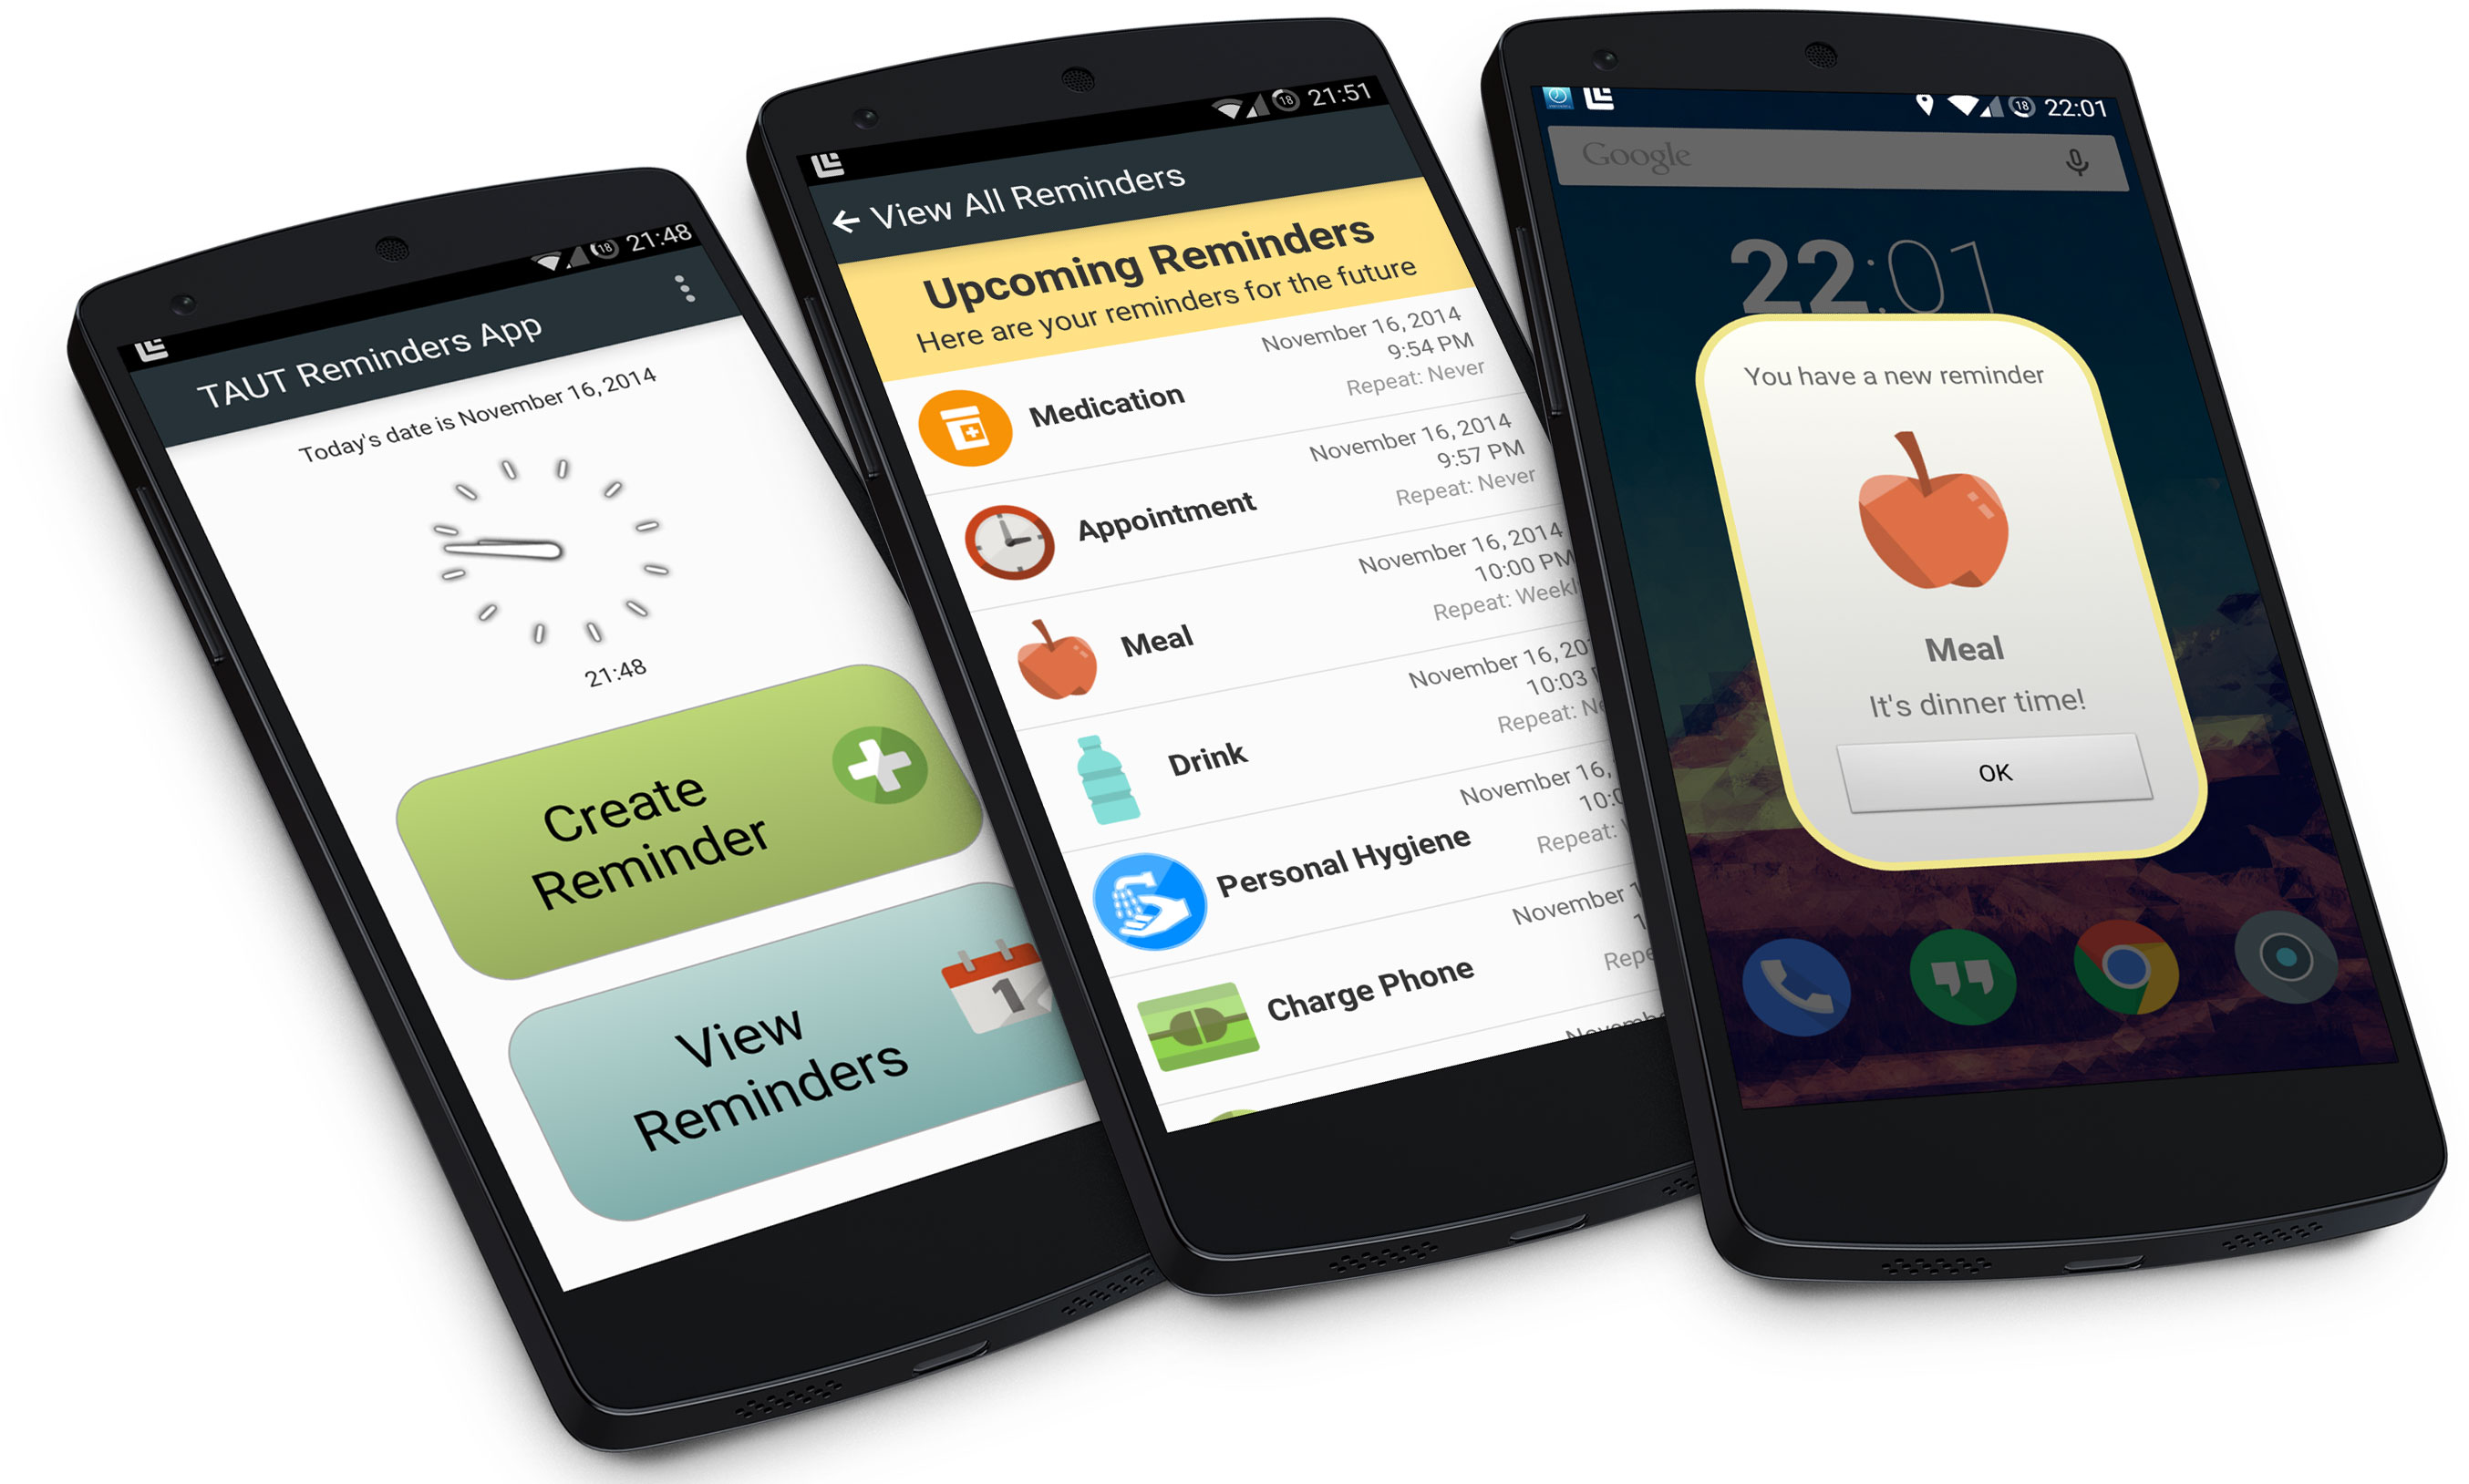
\includegraphics[scale=0.13, angle=0]{Files/treatment-study-1/figures/device-app-screenshots}
        \caption{Home screen, Reminder List and Reminder Delivery Popup screens as displayed on Nexus 4 devices.}
        \label{fig: taut-devices}
\end{figure}

\subsubsection{Creating a Reminder}
The reminders can be created and maintained by the PwD, or by a proxy, such as a caregiver or family member. Using the wizard style approach, the user is guided through the procedure, confirming their choices at each step, as shown in Figure \ref{taut-remindercreation}. Each reminder can be attributed to one of seven ADL types (Meal, Drink, Medication, Hygiene, Appointment, Other, Charge Phone).
The reminders are temporal based, and so the user is asked to confirm the date and time they wish to receive the reminder (Figure \ref{fig: remindercreate-time}), which can also be configured to repeat on a daily, weekly, monthly or custom pattern (Figure \ref{fig: remindercreate-repeat}). At the end of the process, the user is asked to confirm their choices, as per the usability guidelines mentioned earlier.
To provide additional functionality, the ability to record audio messages has also been included. In a similar study, it was noted that coupling voice-based audio recordings with textual descriptions were more effective than video based reminders for PwD \cite{ONeill2010}.

\begin{figure}[h]
    \centering
    \begin{subfigure}[t]{0.3\textwidth}
        \centering
        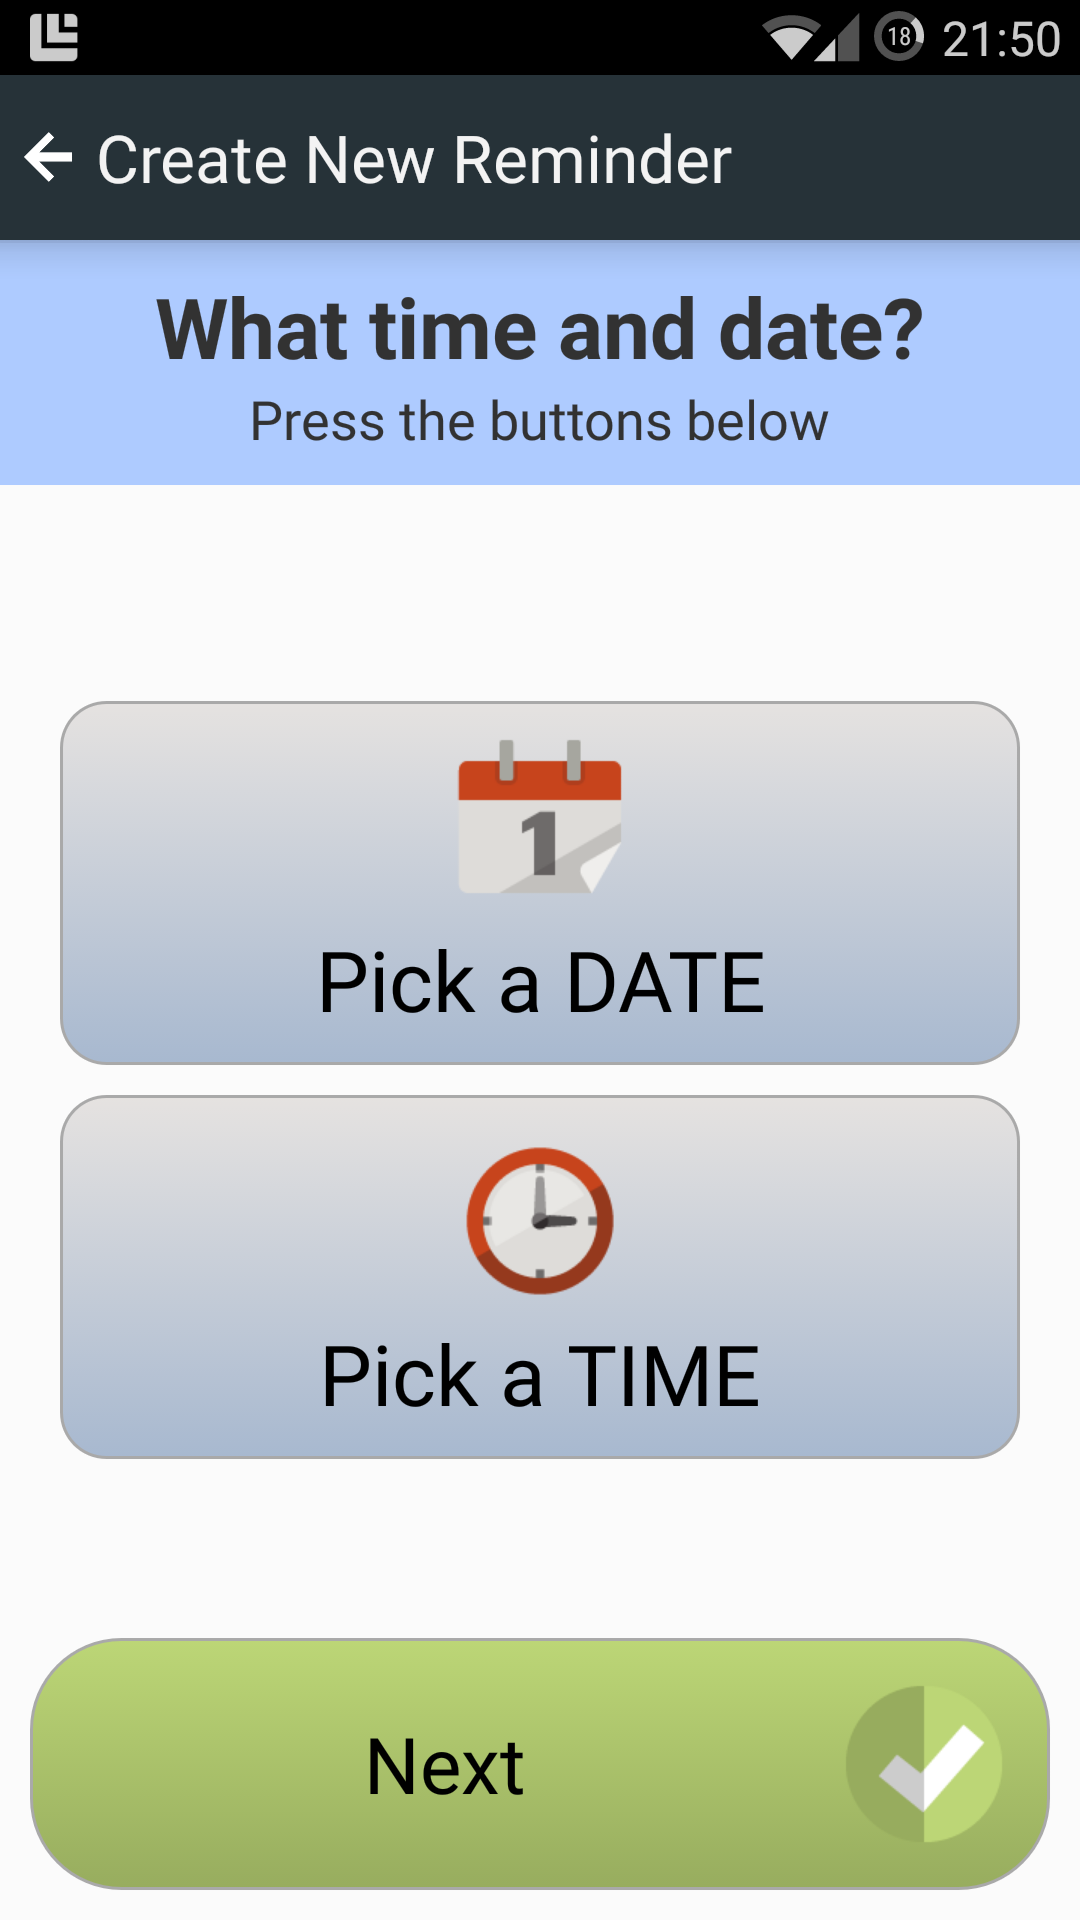
\includegraphics[width=\textwidth]{Files/treatment-study-1/figures/app-remindercreate-1}
        \caption{Date and Time selection screen}
        \label{fig: remindercreate-time}
    \end{subfigure}
    \hfill
    \begin{subfigure}[t]{0.3\textwidth}
        \centering
        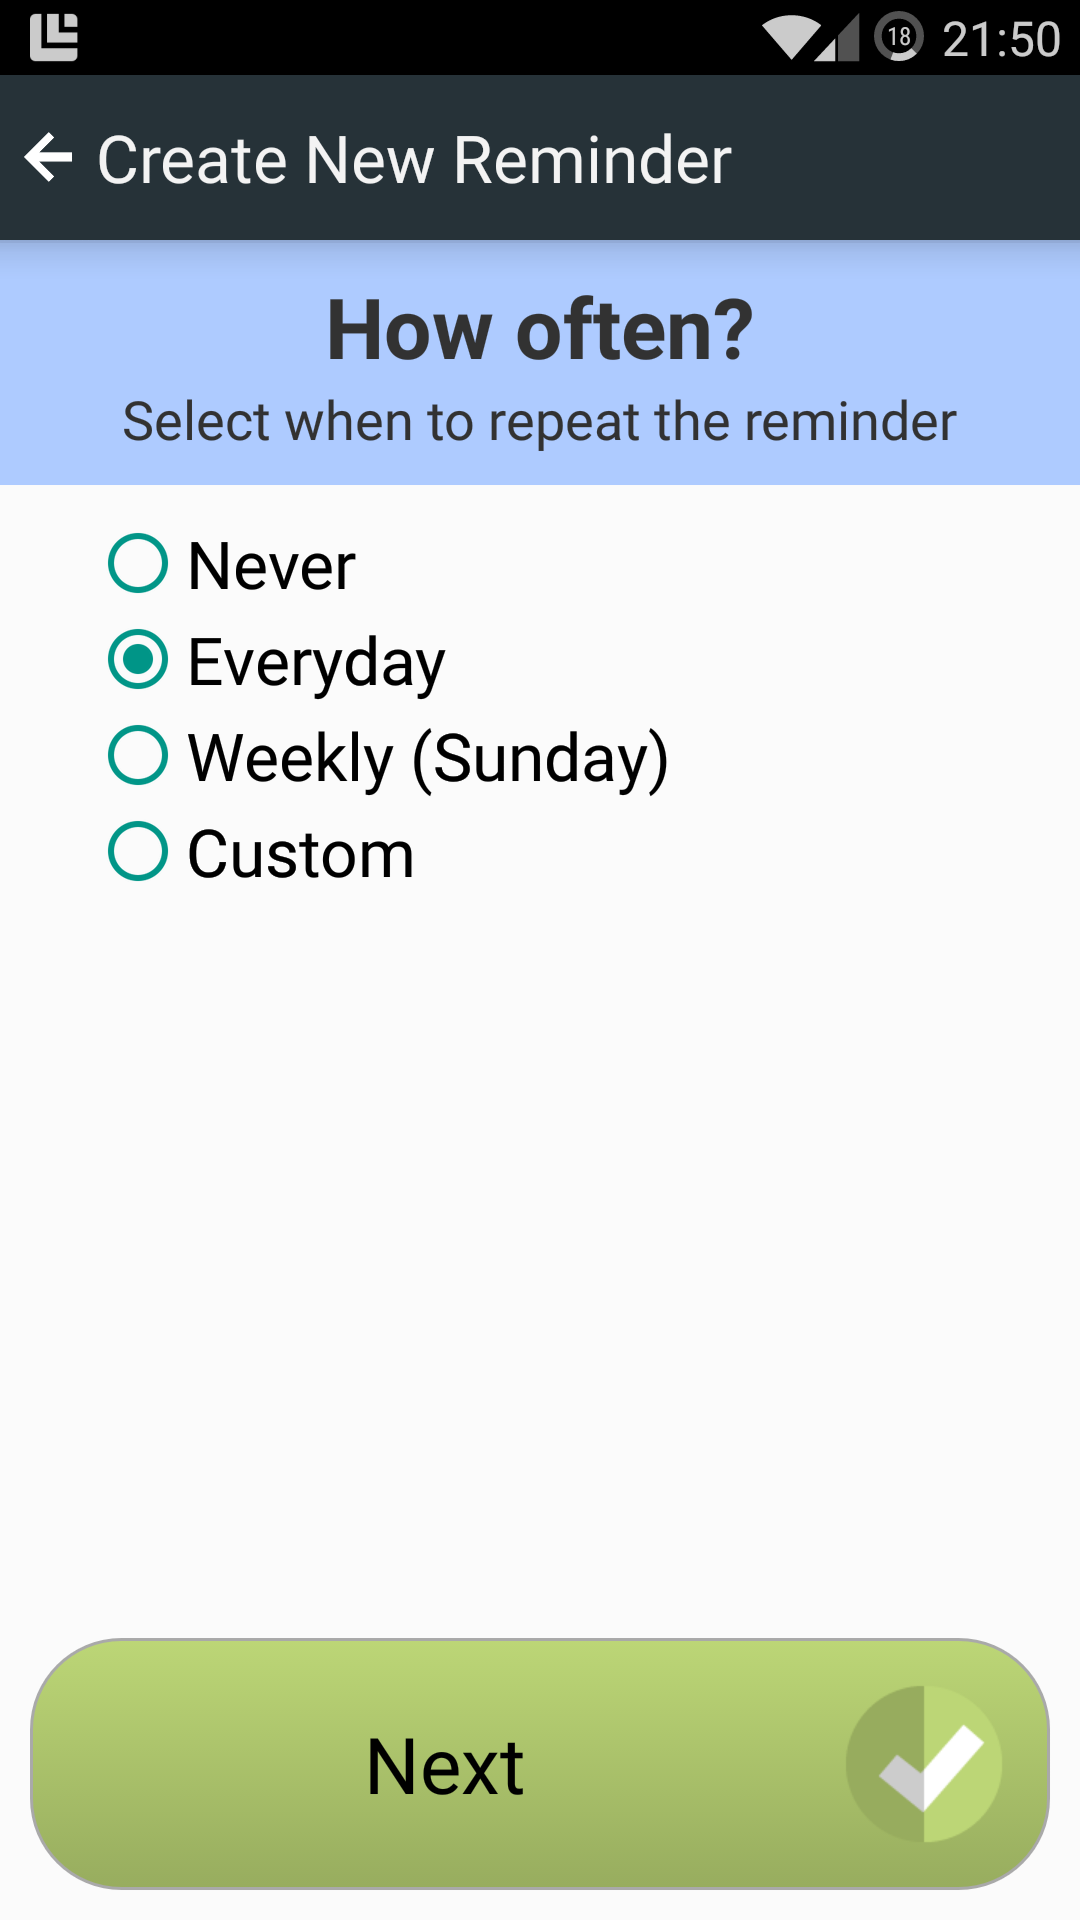
\includegraphics[width=\textwidth]{Files/treatment-study-1/figures/app-remindercreate-type}
        \caption{Repeat Selection}
        \label{fig: remindercreate-repeat}
    \end{subfigure}
    \hfill
	\begin{subfigure}[t]{0.3\textwidth}
        \centering
        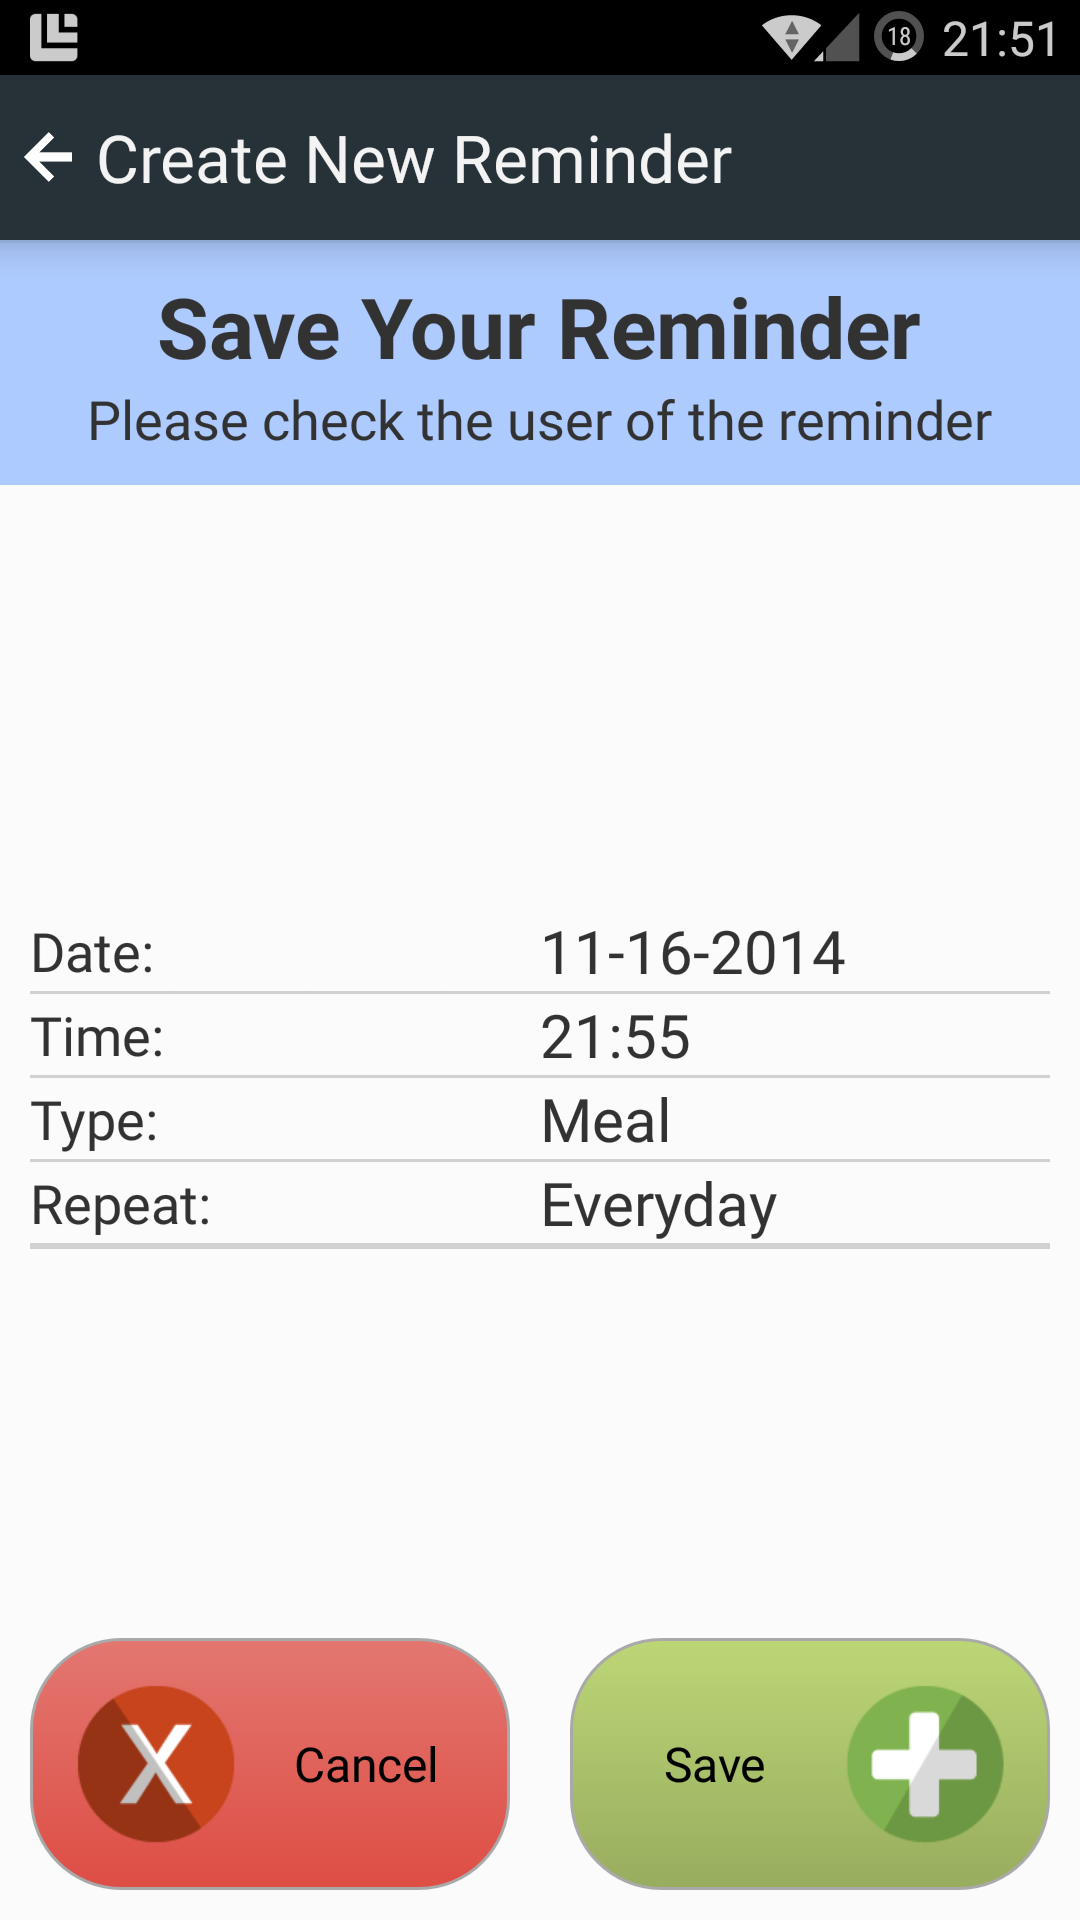
\includegraphics[width=\textwidth]{Files/treatment-study-1/figures/app-remindercreate-confirmation}
        \caption{Confirmation of selected settings}
        \label{fig: remindercreate-confirmation}
    \end{subfigure}
    \caption{Step-by-step reminder creation making use of consistent UI elements, bold text and pastel colours.}
    \label{fig: taut-remindercreation}
\end{figure}

When each reminder was created, a Reminder object (Listing \ref{code: reminderobject}) was stored on the devices local SQLite database, and displayed to the user in the View Reminders screen (Figure \ref{fig: taut-reminderslist}).

\begin{listing}[ht]
\inputminted[
frame=lines,
framesep=2mm,
baselinestretch=1.2,
linenos
]{java}{Files/treatment-study-1/code/Reminder.java}
\caption{Java implementation of a Reminder object.}
\label{code: reminderobject}
\end{listing}
%VIVA: it is probably too late now,  however,  a software architecture or class diagram would maybe have been useful.  Perhaps yu could prepae this after you submit.
\subsubsection{Reminder Delivery} \label{subsubsection: android-alarmmanager}
The delivery mechanism of the reminders makes extensive use of Android's AlarmManager class \cite{GoogleAndroid2016}, enabling each reminder to become a system service. Upon the introduction of Android API 19 (Kit Kat), alarm delivery is inexact, as the operating system will shift alarms in order to minimise wake-ups and battery use. To counter this, the app was explicitly designed to disable the CPU's wake locks as long as the alarm receiver was executing. This guaranteed that the phone would not sleep, or allow another process to interrupt, until each reminder has been delivered, at the cost of battery life.
Each reminder, when delivered, was displayed as a popup dialog box as shown in Figure \ref{fig: taut-reminderpopup}. The popup contained an icon indicating the type of ADL and a textual description of the action the user should perform. As per the recommendations by \citeauthor{CenterforPersonswithDisabilities2015} \cite{CenterforPersonswithDisabilities2015}, a melodic audible tone also accompanied the reminder’s visual delivery.

\subsubsection{Reminder Acknowledgment}
Upon delivery, the user has a time window of 60 seconds in which to acknowledge the reminder. After which, the popup dialog closes, the tone stops playing, and the reminder is logged as ‘missed’. If acknowledged within the 60 seconds the reminder is logged as ‘acknowledged’ and the popup closes. The time taken to acknowledge each reminder instance is also logged.
For voice-based messages, delivery is altered slightly: The user has 60 seconds in which to acknowledge the reminder by playing the voice message. They can re-listen to this voice message as many times as they wish to ensure clarity.
Upon the delivery of each reminder, an acknowledgement object is created, containing a copy of the original reminder object (Listing \ref{code: acknowledgementobject}). In addition to the acknowledgement status of the reminder the object contains the uniqueId of the user, the time taken to acknowledge (if acknowledged), the battery level percentage at the point of delivery, and if an audio reminder the number of times the message was listened to.

\begin{figure}[]
    \centering
    \begin{subfigure}[t]{0.48\textwidth}
        \centering
       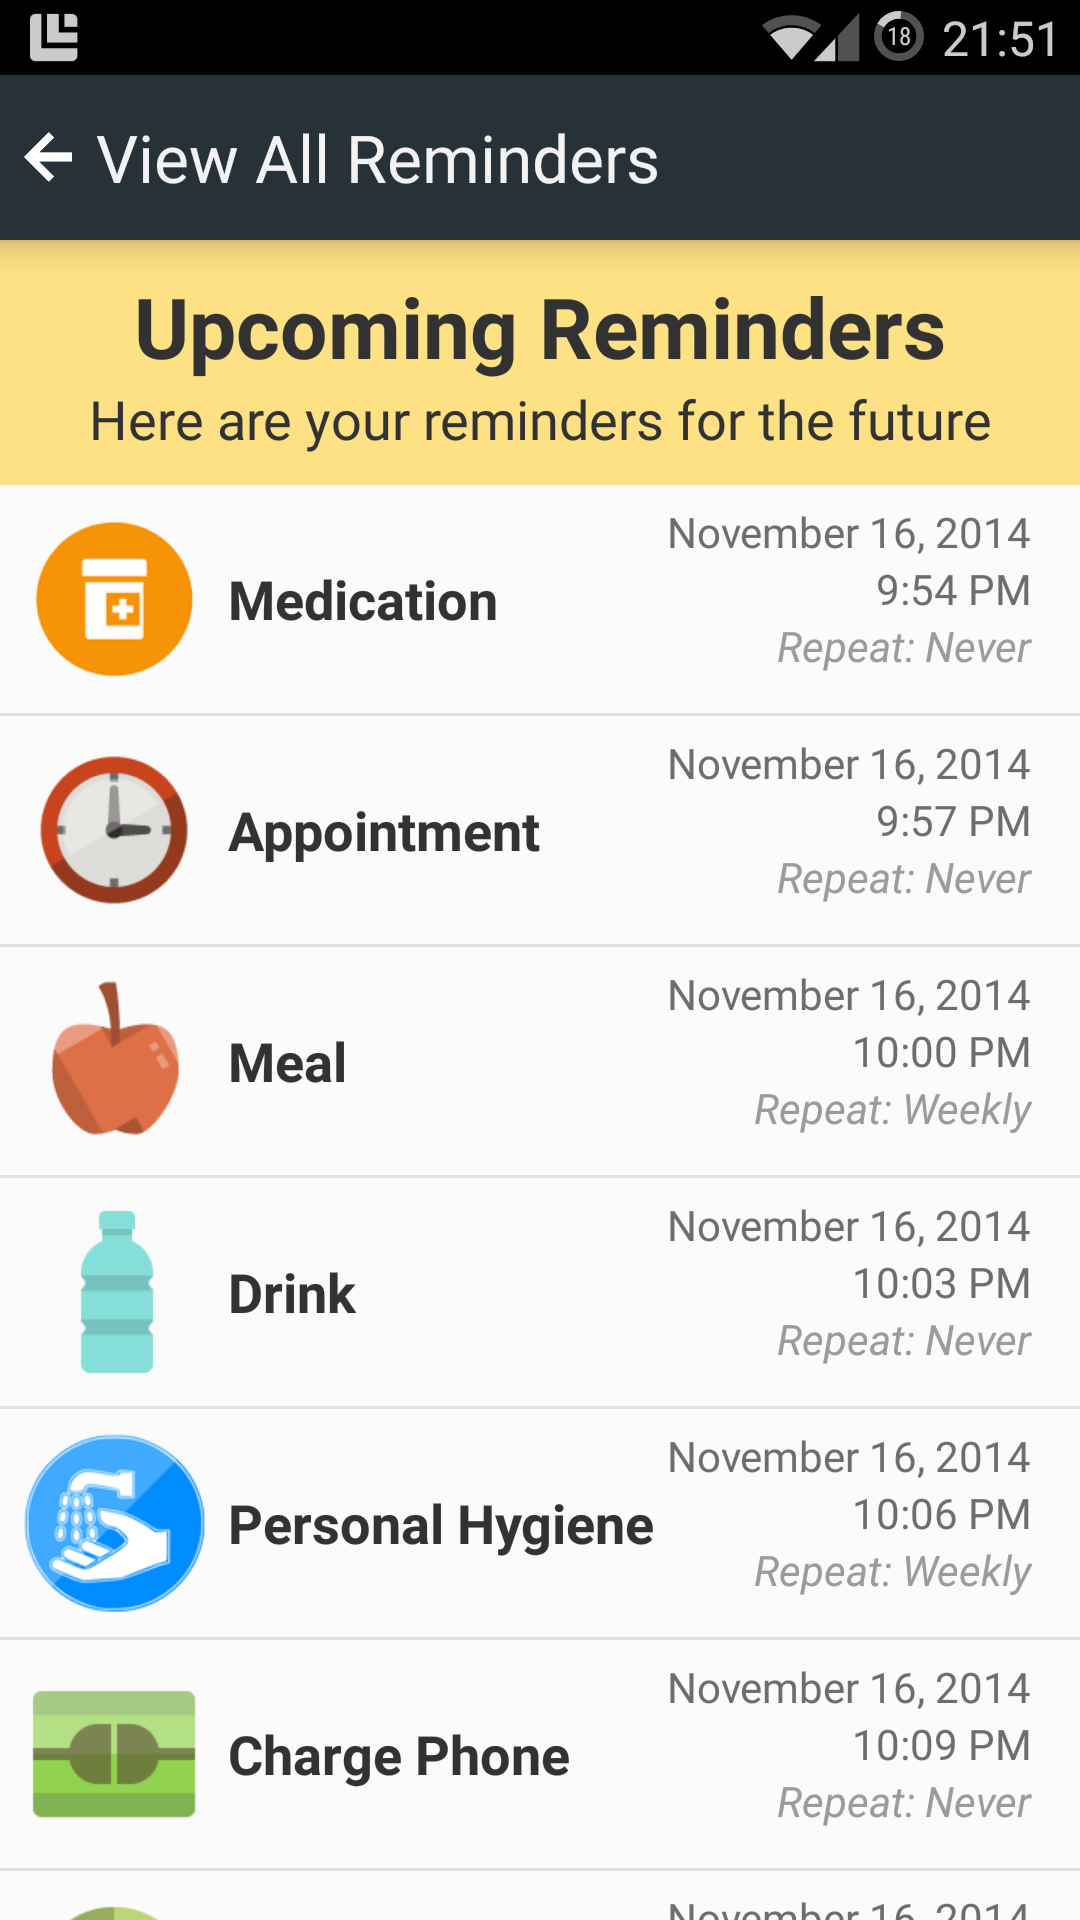
\includegraphics[width=\textwidth]{Files/treatment-study-1/figures/app-reminderslist}
        \caption{View reminders screen displaying all reminders scheduled to be delivered in the future.}
        \label{fig: taut-reminderslist}
    \end{subfigure}
    \hfill
     \begin{subfigure}[t]{0.48\textwidth}
        \centering
      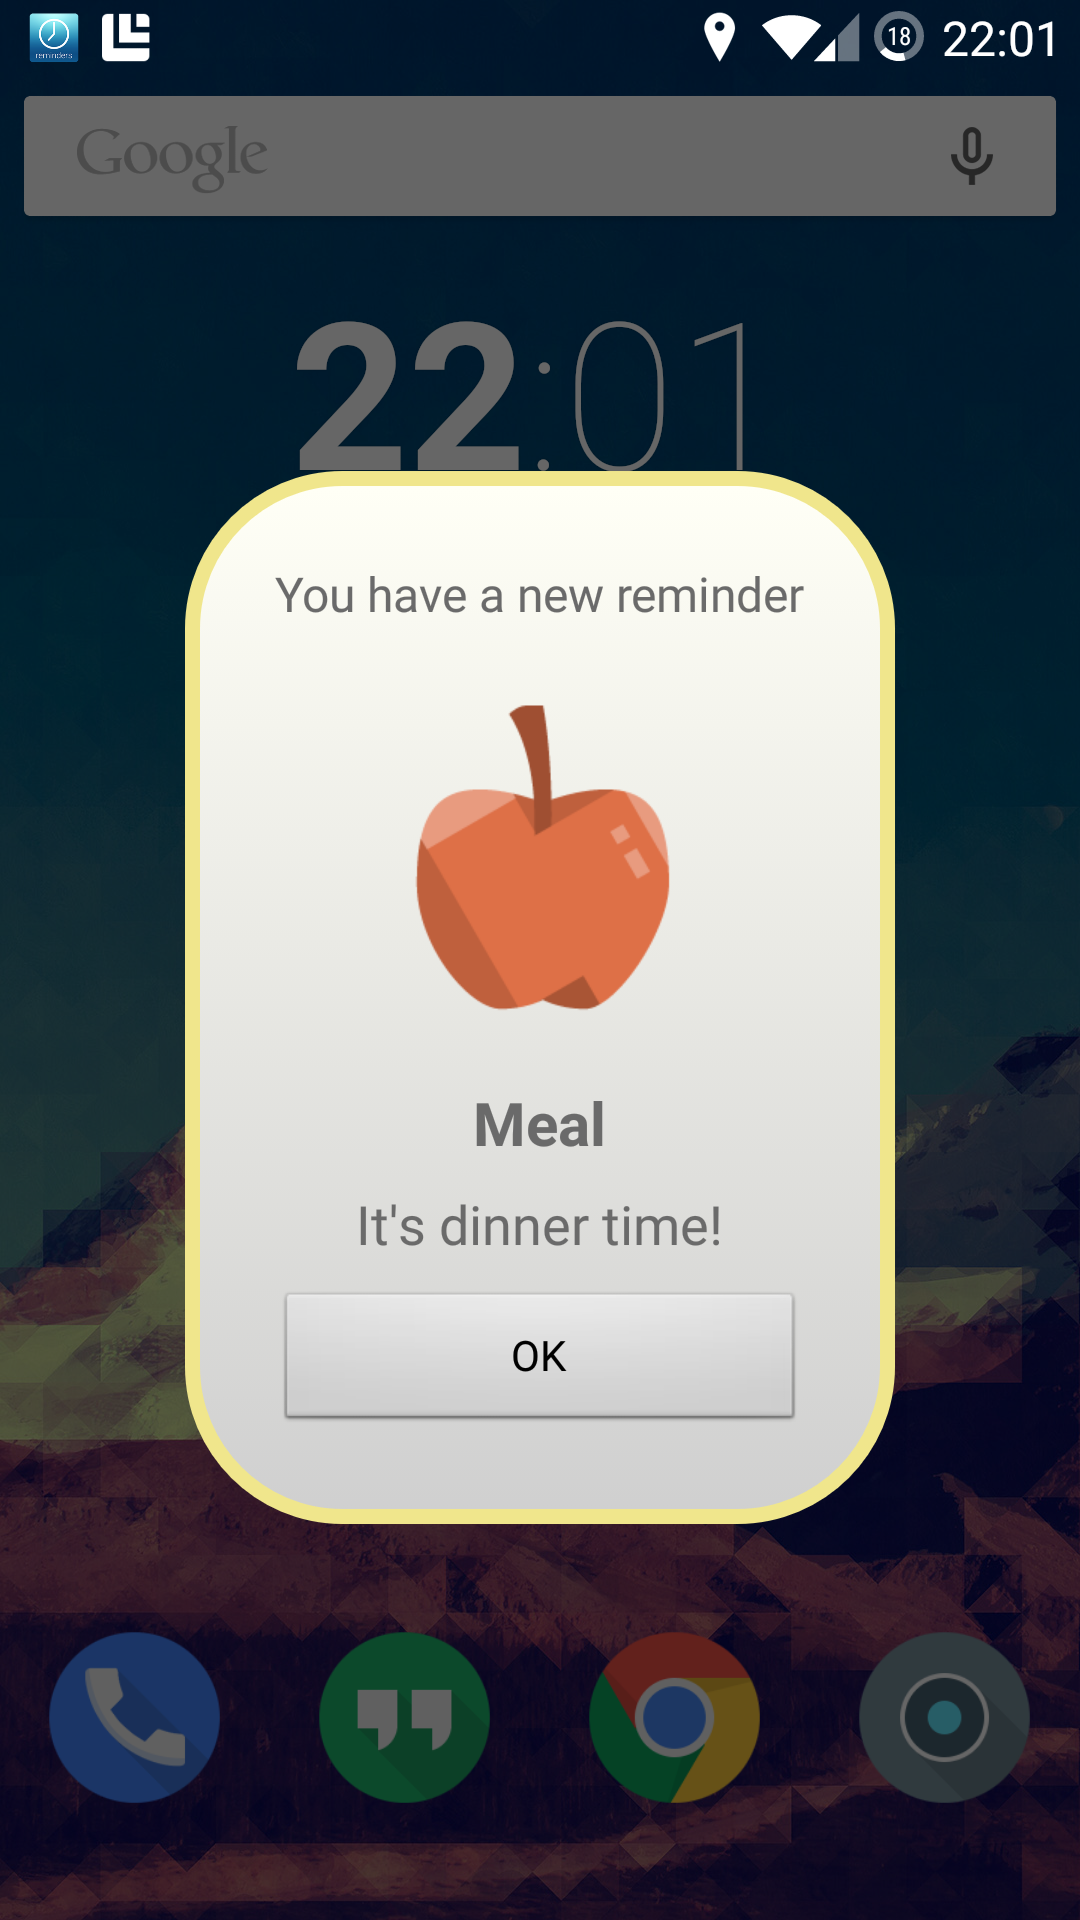
\includegraphics[width=\textwidth]{Files/treatment-study-1/figures/app-reminderpopup}
        \caption{Reminder delivery as a dialog popup with accompanying sounds.}
        \label{fig: taut-reminderpopup}
    \end{subfigure}
      \caption{Reminders scheduled and delivery popups.}
    \label{fig: taut-reminderlist-delivery}
\end{figure}

\begin{listing}[ht]
\inputminted[
frame=lines,
framesep=2mm,
baselinestretch=1.2,
linenos
]{java}{Files/treatment-study-1/code/Acknowledgement.java}
\caption{Java implementation of an Acknowledgement object. The acknowledgement object also contains an immutable copy of the original Reminder object that created it.}
\label{code: acknowledgementobject}
\end{listing}

\subsection{Usage Data Collection Tool}
To support the collection of insightful usage data for the TAUT project, the app records various metrics based upon a user’s interactions with the app. These metrics can be categorised as usage behaviours and reminder data.
\newline \textbf{Usage behaviour} relates to a user’s active engagement with the app, such as how the user navigates the screens of the interface, how long they spend on each screen and how often they launch the app.
\newline \textbf{Reminder data} contains all the relevant information on previously delivered and future scheduled reminders. From high-level analysis of reminder data it is possible, for each individual, to establish the most common ADL type that requires assistance, establish their preferences for voice or text-based reminders and also view who typically creates the reminders.
From this data, it is also possible to perform analysis on the time taken to acknowledge a reminder as shown previously in Listing \ref{code: acknowledgementobject}. From this metric, it is possible to calculate a baseline or average response time and observe for sudden or atypical increases. It is hypothesised that a change in this value, indicating slower reaction times, has the potential to be used as an indicator of further cognitive decline, or disengagement from the technology \cite{Phillips2013}.

\subsubsection{Reminder Acknowledgement}
Regarding adoption, and efficacy of the reminder device, the most pertinent of the data recorded is within the delivered reminders. Analysis of the delivered reminders exposes the number of reminders missed or acknowledged, from which a single metric of an individual’s adherence to the system can be established. To avoid the inclusion of false negatives, the app can detect if a reminder has been missed due to the device being in a powered off state, rather than a lack of human interaction. These instances are logged as a separate value.
The use of this acknowledgement status plays a key role in labelling contextual data observed from the sensors.

\subsection{Contextual Observation}
In the study a key focus is to observe how the PwD interacts with the device, whilst the author hypothesises that contextual observations may be used to make these interactions more consequential and effective. A key component of this approach is to observe the contexts at the time of interaction with the device, and specifically around the point in time when reminders are acknowledged or missed.
\subsubsection{Observation Window}
The time period in which the reminders are scheduled for delivery presents a suitable window in which to observe controlled and understood contextual information. By observing the contexts in this window it may be possible to associate certain sensor states with acknowledged or missed reminders.
For the purposes of this study the app has been configured to record the raw outputs of all available sensors 3 minutes prior to a reminder being delivered, and continues to record data for 3 minutes after the reminder has been delivered. This creates a number of sensor output files, with a total recording duration of 6 minutes, for each available sensor.
Unix timestamps (ms) are used to enable synchronicity across the various recordings.
During initial beta testing of the app, it was shown that a 6 minute window provided a good balance of contextual information, whilst keeping file size relatively low \cite{Hartin2014-EMBC}. A typical set of 6-minute recordings from the Moto G, using all available sensors, records at approximately 130KB/min.

\subsection{Sensor Platforms}
As the app has been developed for android smartphones, it is possible to utilise a variety of on-board sensors to observe and record contextual information. The android platform groups their array of available sensors into 3 main categories: motion, positional and environmental.

\subsubsection{Motion}
Within the android platform there are 2 core hardware based motion sensors, the accelerometer, and the gyroscope. The sensors capture acceleration and rotation forces along 3 dimensions, or axes. These sensors measure acceleration forces and rotational forces along three axes. The category also includes gravity sensors and rotational vector sensors.
In the android platform, where a hardware sensor is missing, in many cases a simulated sensor can be generated from the input of another, e.g. using the accelerometer and magnetometer to simulate a gyroscope.
Previous studies have relied heavily upon the use of accelerometers for the classification of physical activities, and gyroscopes are often use in conjunction, strengthening the classifiers \cite{Wu2012, Preece2009}. In many cases, these sensors require additional processing to extract relevant information. For example, the accelerometer, measures the acceleration applied to the device, which\textit{includes the force of gravity}. Many previous studies using standalone accelerometers must calibrate and apply a high-pass filter to isolate the true rate of acceleration \cite{Ferraris1995}. The android platform makes it possible to record this true acceleration (minus gravity) directly from the device, with the caveat that it always has an offset, which needs to be removed through calibration.

\subsubsection{Positional}
Positional sensors provide information that can determine the position of the device. These consist of the magnetometer, the orientation sensor and the proximity sensor.
The magnetometer provides information regarding orientation across 3-axes. The orientation sensor is an emulated sensor using calibrated data from the raw magnetometer data, and provides provides the azimuth (yaw), pitch, and roll values.
Magnetometers have been used in combination with accelerometry data for the classification of human activities in similar studies \cite{Zhang2015,Catal2015}.
The proximity sensor provides a measure of distance between the sensor and an object. The sensor is forward facing, and is primarily used by the operating system to turn the screen off if the sensor is occluded, signifying that the user has the phone close to their face, or in their pocket, to avoid accidental presses. In this study, however, the proximity sensor is expected to provide refining information in a number of scenarios. E.g. movement is observed in the accelerometer, and the proximity sensor shows the phone is not occluded. This may indicate that the phone is in the user's hand, resulting in an opportune time to deliver a reminder \cite{Hoseini-Tabatabaei2013}. Unlike the accelerometer and magnetometer, who return multidimensional arrays of data, the proximity sensor returns a single value when polled.

\subsubsection{Environmental}
Environmental sensors aim to observe various environmental properties, including illumination, air temperature, air pressure, and humidity. To perform these readings, the smartphone requires a photometer, thermometer and barometer, all of which are hardware based. As such, the inclusion of these sensors is scarce, with the light sensor (photometer), being the most commonly included by device manufacturers. As with the proximity sensor, the light sensor returns a single illuminance (lux) reading when polled. These sensors require no calibration. The values from these sensors are not expected to yield sufficient data for an accurate context aware system, however, their fusion with the other sensor types may refine and influence a classifier.


\subsection{Device Consistency} \label{subsection: taut-deviceconsistency}
A downside to developing for the android platform, is that the selection of sensor modalities is at the manufacturers discretion. This means that the number of sensor platforms which are available vary across devices. Given that this is a scientific study, steps were taken to ensure consistency across the cohort. Taking into consideration the cost to sensor ratio, it was decided that the Motorola Moto G smartphone was an appropriate choice for the study. The Moto G is equipped with an accelerometer, magnetic field sensor, proximity sensor, light sensor and a GPS receiver chip. Ulster University's Ethical Committee approved the use of all sensors, with the exception of the GPS, due to privacy concerns. As such, the remaining 4 sensors were used, which still address the 3 main sensor categories of the android platform, and are consistent with the sensors used in similar studies \cite{Poppinga2014}.

\subsection{Internet Connectivity}
Initial analysis of the intended study cohort's location uncovered sparse internet connectivity, both in the home and via mobile networks. This influenced the design of the data model, resulting in an offline-first app, storing all recorded data, both usage (SQLite) and sensor (CSV), on the local disk, negatively impacting data redundancy. To mitigate the risk of losing data, the app was also programmed to be opportunistic with connectivity. If an internet enabled connection was detected (3G, LTE, or Wi-Fi), the app would attempt to send the reminder acknowledgement data to a remote MySQL server with a low overhead in JSON format. The raw sensor data would be to large to send via an opportunistic connection, and so physical access to the handset would still be required to retrieve the data.

\section{Testing and Evaluation}
To ensure that the developed application and context-aware sensor framework was fit for purpose, the app was deployed to an internal testing and evaluation cohort at Ulster University. Ethical approval to perform the study was granted by Ulster University's Research Ethics Committee (HARTIN001).

\subsection{Objectives}
The testing study had the following objectives:
\begin{itemize}[noitemsep,topsep=0pt]
  \item to investigate the use of the smartphone’s embedded sensors to detect the user’s movement, location and environmental contexts.
  \item to investigate the correlation between the contextual sensor information and observed notification adherence.
  \item to identify the optimal sensor types and combination permutations to provide useful contextual sensor information.
  \item to evaluate the usability of the smartphone platform to provide and gather information from the user.
  \item to create an openly available data set to publish within the research community.
\end{itemize}

\subsection{Recruitment}
Recruitment was performed by email, sent to Engineering and Computing faculty members at Ulster University. 9 healthy members of the Smart Environments Research Group responded and were recruited for the study (Median age: 27). These participants will hereafter be referred to as the test cohort (TC).

\subsection{Study Design}
The study was designed to be a non-randomised controlled study, with a duration of 7 days. Participants were asked to perform a single compulsory task: to set a notification for a time that was convenient to them. If the participants found the notifications useful they may set as many as they wish. In order to investigate variations in context throughout the day, the participants were asked to use the app to assist them with scheduling meals, appointments and other general activities of daily living.

\subsection{Outcome Measures}
The outcome measures of the study included quantifying the number of reminders set by each participant, calculation of their acknowledgement rate and the types of reminders set. In addition offline analysis, labelling, and initial classifier modelling was performed on the sensor data to ensure the data was fit for purpose. Details of data modelling and classification results are detailed in Section \ref{section: taut-results}.

\subsection{Results}
Having collected the data from the TC, adoption, usage and sensor data were analysed.

\subsubsection{Adoption and Usage}
As a data collection tool the app performed its intended role. An overview of the reminder statistics are presented in Table \ref{tbl: taut-pilot-reminders}. In total 223 reminders were scheduled to be delivered during the evaluation period, of which a total of 73\% (163) were acknowledged with a mean response time of 12.38 seconds. Upon further analysis it was discovered that 23.33\% (14) of the missed reminders were due to the device being in a powered off state. Many of reminders were set to repeat daily at the same time, thus potentially increasing their chances to be acknowledged \cite{Hartin2014-EMBC}.
%VIVA: Question - Why does this increase the chances to be acknowledged?

\begin{table}[h]
\centering
\caption{Reminder acknowledgement statistics for internal testing and evaluation study}
\label{tbl: taut-pilot-reminders}
\resizebox{\textwidth}{!}{%
\begin{tabular}{@{}lllllll@{}}
\toprule
Participant & \begin{tabular}[c]{@{}l@{}}Reminders \\ Set\end{tabular} & \begin{tabular}[c]{@{}l@{}}Acknowledged\\ (count)\end{tabular} & \begin{tabular}[c]{@{}l@{}}Acknowledged\\ (\%)\end{tabular} & \begin{tabular}[c]{@{}l@{}}Missed\\ (count)\end{tabular} & \begin{tabular}[c]{@{}l@{}}Missed\\ (\%)\end{tabular} & \begin{tabular}[c]{@{}l@{}}Mean \\ response\\ time (s)\end{tabular} \\ \midrule
P01 & 47 & 32 & 68.09\% & 15 & 31.91\% & 14.26 \\
P02 & 9 & 6 & 66.67\% & 3 & 33.33\% & 16.32 \\
P03 & 8 & 8 & 100.00\% & 0 & 0.00\% & 11.89 \\
P04 & 20 & 15 & 75.00\% & 5 & 25.00\% & 11.56 \\
P05 & 7 & 6 & 85.71\% & 1 & 14.29\% & 5.6 \\
P06 & 39 & 35 & 89.74\% & 4 & 10.26\% & 12.96 \\
P07 & 34 & 25 & 73.53\% & 9 & 26.47\% & 9.03 \\
P08 & 17 & 12 & 70.59\% & 5 & 29.41\% & 14.61 \\
P09 & 42 & 24 & 57.14\% & 18 & 42.86\% & 15.17 \\ \midrule
Total & 223 & 163 & 686.47\% & 60 & 213.53\% & 96.23 \\
Mean & 24.7 & 18.1 & 73.09\% & 6.6 & 26.91\% & 12.38 \\ \bottomrule
\end{tabular}
}
\end{table}

\subsubsection{Sensor Recording}
The app also fulfilled its function as a context-gathering tool, recording 6-minute windows of sensor data for each of the reminders delivered. Each time-series based recording (accelerometer and magnetometer) required 2.6 MB of hard disk space. When compressed, the size was reduced to 430kb.
Rudamentary analysis of the acknowledged reminders observed in the TC cohort shared a similar pattern. The pattern which was observed was if the device was static, showing minimal movement in the accelerometer signal, and also reading low light levels, the reminders were predominately acknowledged.
 A post-evaluation questionnaire, performed by a subset of the TC (n=5), revealed that this may be due in part to the similarity of the activities they performed during the study, such as working at a desk or attending meetings, performed daily by 100\% and 80\% of the respondents respectively \cite{Hartin2014-EMBC}.
Placement of the smartphone was also similar across the respondents, with their smartphones placed on their desks (100\%), or in their trouser pockets (left pocket: 40\% and right pocket: 60\%) for the majority of the use cases. The questionnaire also revealed that the top 4 reasons for missed reminders within the cohort were:

\begin{enumerate}[noitemsep,topsep=0pt]
	\item Otherwise engaged in an activity (100\%)
	\item Not carrying smartphone (80\%)
	\item Did not hear the notification (60\%)
	\item Reminder was not loud enough (40\%).
\end{enumerate}

\subsection{Observations and Improvements} \label{subsection: improvements}
As highlighted in Section \ref{subsection: taut-deviceconsistency}, the trial study cohort's intended device was the Motorola Moto G, from which all development and pre-release testing was based. Upon deploying the app to each participant's personal smartphone for the evaluation a number of observations were made.
Firstly, those with older devices noticed increased battery drain and slower average response times for other apps, when future reminders were scheduled. Replicating these conditions after the study uncovered the cause to be the implementation of the reminder delivery mechanism. As noted earlier in Section \ref{subsubsection: android-alarmmanager}, the android platform's delivery of time based notifications is accurate, however, not to a degree of milliseconds. In an effort to ensure perfect synchronicity between the reminder delivery, and the midpoint of the sensor recording, the author used a thread that continuously checked the current unixtime against that of the upcoming reminder. Whilst acceptable in theory, the inefficiency of this approach was noted on less powerful devices, and was subsequently removed before deployment to the main demented study cohort. To ensure synchronicity between sensor recordings and the reminder delivery in later versions, the exact unixtime to a millisecond precision is recorded as part of the reminder object, and synchronisation is performed retrospectively.
The second observation was made during the analysis of sensor data. As stated earlier, it is to the discretion of the handset manufacturer which hardware they include in their devices. Amongst the TC, there was an observable difference in the calibration offset and sampling rates of the accelerometer data. The reasons for this, and methods to rectify are presented later in the Chapter, with particular focus in the pre-processing section.

\section{Study with PwD}
Having improved the performance and stability of the app based upon the findings during testing, the app was then deployed to the intended study cohort, 30 PwD based in Cache County, Utah.

\subsection{Study Design}
The app was designed as the principle technology component for the TAUT project, a collaborative project between Utah State University (USA), the University of Utah (USA) and Ulster University (UK).
The project integrates data from two large databases, the Cache County Study on Memory in Aging (CCSMA) and the Utah Population Database (UPDB) in an effort to build a user profile. The CCSMA is a longitudinal, population based study of AD and other dementias, which has followed over 5,000 elderly residents of the Cache County, Utah (USA) for over twelve years (1995-2007) \cite{Tschanz2013}. The UPDB contains genealogical, medical, vital and demographic records, with full coverage of medical information spanning the past 20 years for over 7 million people.

\subsubsection{Recruitment}
From the integrated dataset, a subset of 125 individuals showing the greatest decline in cognition, evaluated by a 3MS \cite{Tschanz2002}, were identified as being suitable for the study. From this 125, 30 were screened and recruited for the study (Figure \ref{fig: taut-recruitment}). These participants are hereafter referred to as the Dementia Cohort (DC).

\begin{figure}[h]
    \centering
        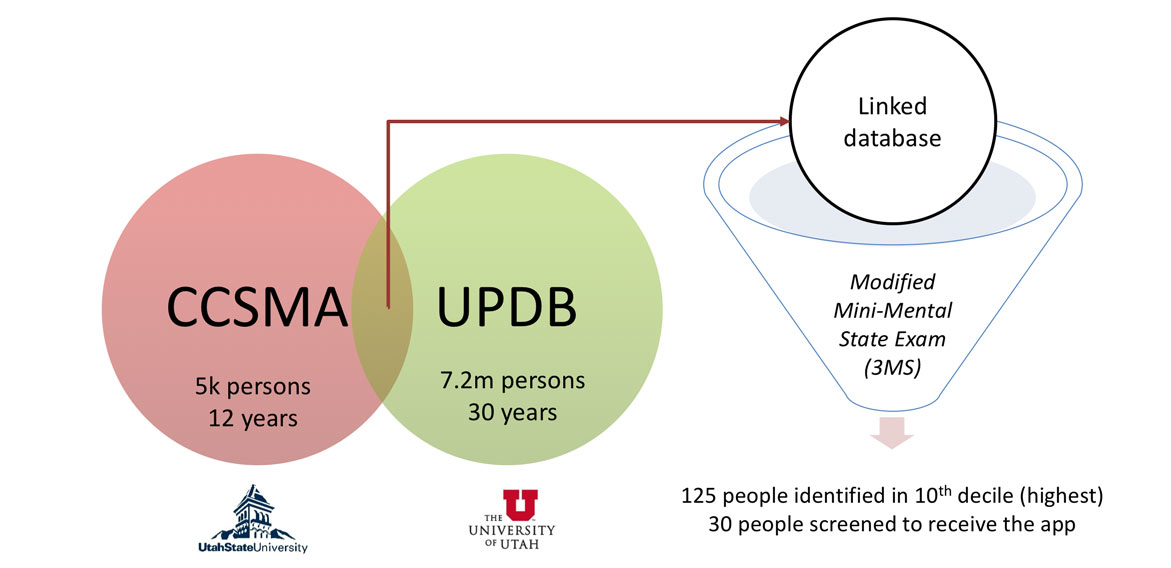
\includegraphics[scale=0.3, angle=0]{Files/treatment-study-1/figures/taut-recruitment}
        \caption{Recruitment from a subset of participants found in both the UPDB and the CCSMA databases.}
        \label{fig: taut-recruitment}
\end{figure}

\subsection{Deployment to Cohort}
Each smartphone device was preloaded with the TAUT app and physically delivered to each participant by a small team of research associates based at Utah State University, Utah. The study participant, and if possible their carers, were provided with a short training demo as to how the app operated, including instructions how to set, view and acknowledge reminders, and how to charge the device.

\subsection{Post-Study Data Retrieval}
It was understood that the DC would have restricted access to the internet. As stated earlier, in anticipation of this, all data was stored locally on the device, with opportunistic syncing to an online database. A number of visits were scheduled with the cohort to permit the retrieval of sensor data during the study, with the aim of producing snapshots of progress throughout the study, however, many participants were unavailable at their scheduled times. For the sensor data that was retrieved, preliminary and exploratory analysis was performed \cite{Hartin2014-WAGER}, however, the datasets were sparse and heavily unbalanced at this point.
At the study close, all the devices, with the exception of 2 which were lost by the study participants, were retrieved, and the raw data was downloaded for processing.

\section{Adoption and Usage by PwD}
This Section will cover the user adoption and usage of the app, with detailed analysis on context-aware results covered later in the Chapter.
Encouraging usage was observed in the initial month, when one of the participant's who had internet access in the home synchronised their data. At this time, the total number of reminders delivered to the user was 215, with a mean acknowledgement rate of 58.1\% \cite{Hartin2014-EMBC}. Upon the study close, however, the total number of reminders set to be delivered to all users was 8881, with a mean acknowledgement rate of 19.2\% (n=1686). It is important to note that the calculation of this metric includes reminders which were missed due to the phone being in a powered off state. Removing these instances resulted in a total of 6289 reminders being truly delivered by the phone, with a mean acknowledgement rate of 26.8\% (\textit{(1686/6289)*100}). This statistic is somewhat skewed by the non-adopters in the study \cite{Cleland2014-IWAAL}. For adopters of the platform, the mean individual acknowledgement rate was 39.2\%. Full statistics for each participant can be found in Table \ref{tbl: taut-reminder-stats} and represented visually in Figure \ref{fig: reminder-stacked-stats}.

\begin{table}[h]
\centering
\caption{Reminder acknowledgement statistics for 30 persons with dementia, ordered by total reminders in descending order.}
\label{tbl: taut-reminder-stats}
\resizebox{\textwidth}{!}{%
\begin{tabular}{@{}lllllll@{}}
\toprule
Participant & \begin{tabular}[c]{@{}l@{}}Number of \\ Reminders\end{tabular} & Acknowledged & Missed & Device Off & Acknowledged \% & Missed \% \\ \midrule
P01 & 2874 & 850 & 1728 & 296 & 33\% & 67\% \\
P02 & 1335 & 379 & 937 & 19 & 29\% & 71\% \\
P03 & 600 & 364 & 172 & 64 & 68\% & 32\% \\
P04 & 557 & 33 & 219 & 305 & 13\% & 87\% \\
P05 & 531 & 6 & 523 & 2 & 1\% & 99\% \\
P06 & 473 & 4 & 207 & 262 & 2\% & 98\% \\
P07 & 472 & 9 & 222 & 241 & 4\% & 96\% \\
P08 & 426 & 1 & 40 & 385 & 2\% & 98\% \\
P09 & 401 & 6 & 9 & 386 & 40\% & 60\% \\
P10 & 229 & 1 & 194 & 34 & 1\% & 99\% \\
P11 & 225 & 2 & 199 & 24 & 1\% & 99\% \\
P12 & 218 & 5 & 22 & 191 & 19\% & 81\% \\
P13 & 94 & 3 & 19 & 72 & 14\% & 86\% \\
P14 & 76 & 3 & 2 & 71 & 60\% & 40\% \\
P15 & 72 & 6 & 66 & 0 & 8\% & 92\% \\
P16 & 71 & 2 & 4 & 65 & 33\% & 67\% \\
P17 & 49 & 1 & 22 & 26 & 4\% & 96\% \\
P18 & 43 & 2 & 18 & 23 & 10\% & 90\% \\
P19 & 28 & 0 & 0 & 28 & - & - \\
P20 & 2 & 2 & 0 & 0 & 100\% & 0\% \\
P21 & 2 & 2 & 0 & 0 & 100\% & 0\% \\
P22 & 2 & 2 & 0 & 0 & 100\% & 0\% \\
P23 & 2 & 1 & 0 & 1 & 100\% & 0\% \\
P24 & 1 & 1 & 0 & 0 & 100\% & 0\% \\
P25 & 1 & 1 & 0 & 0 & 100\% & 0\% \\
P26 & 0 & 0 & 0 & 0 & - & - \\
P27 & 0 & 0 & 0 & 0 & - & - \\
P28 & 0 & 0 & 0 & 0 & - & - \\
P29 & 0 & 0 & 0 & 0 & - & - \\
P30 & 0 & 0 & 0 & 0 & - & - \\ \midrule
Sum & 8784 & 1686.0 & 4603.0 & 2495.0 & 941.8\% & 1458.2\% \\
Mean & 302.8965517 & 58.1 & 158.7 & 86.0 & 39.2\% & 60.8\% \\ \bottomrule
\end{tabular}
}
\end{table}

It may be noted from the Table that there was a large degree of difference between the two main outcomes: acknowledged and missed. The impact of this in the development of the context-aware reminder system is discussed later in the Chapter.

\begin{figure}[h]
    \centering
        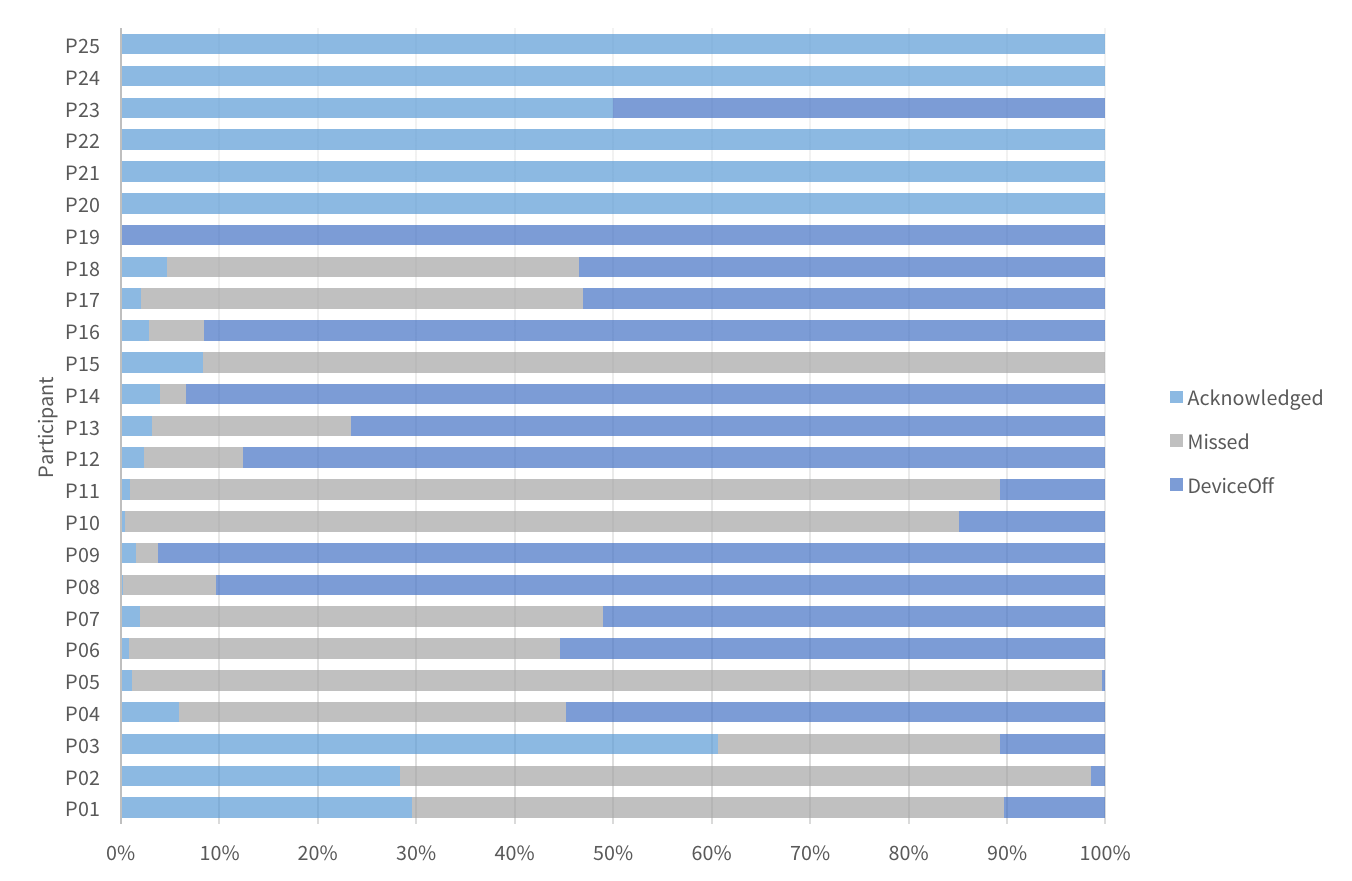
\includegraphics[scale=0.6, angle=0]{Files/treatment-study-1/figures/reminder-stacked-stats}
        \caption{Stacked bar graph showing distribution of scheduled reminders that were Acknowledged, Missed, and Missed due to powered off device.}
        \label{fig: reminder-stacked-stats}
\end{figure}

\subsection{Response Times}
As stated earlier, the time taken to acknowledge a reminder was recorded. It was hypothesised by the author that the change in response time could potentially be correlated with decline of MMSE scores. What was originally observed in the first few months of the study, using the initial data snapshot obtained from the participant who had an internet connection (P03), was that their response times had decreased, as shown in Figure \ref{fig: responsetimedecrease}.

\begin{figure}[h]
    \centering
        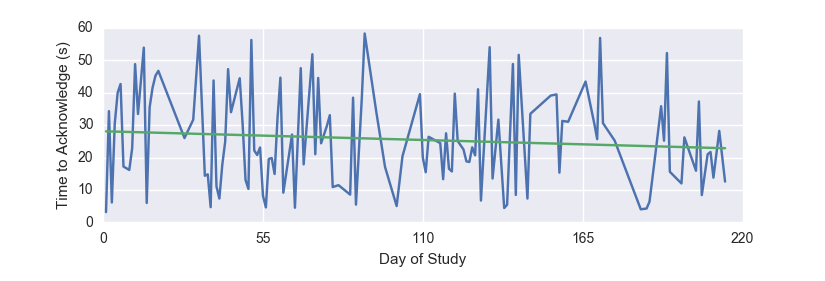
\includegraphics[scale=0.7, angle=0]{Files/treatment-study-1/figures/responsetimedecrease}
        \caption{Example of Participant 03's response times decreasing over study period, indicating adoption and familiarity with platform.}
        \label{fig: responsetimedecrease}
\end{figure}

This particular participant passed away before the official end of the study, and as such, the reason's for their improved response times remains unclear. It is evident however, that the participant adopted the technology, having acknowledged multiple reminders and it is proposed their increased response time was due to increased reliance and reduced device proximity.

At the study close, an exploratory analysis was performed on response times and their change in participants with greater than 5 acknowledged reminders. The results can be found in Table \ref{tbl: response-times}. Regression was performed using the participant's response time against the unixtime of the reminder. From the regression slope it is clear that the majority of users experienced an increase in response times as the study progressed, most notably in P05 and P02. The correlation and fit of this slope, however, is poor.

\begin{table}[h]
\centering
\caption{Response times and regression statistics for participants with greater than 5 acknowledged reminders.}
\label{tbl: response-times}
\resizebox{\textwidth}{!}{%
\begin{tabular}{@{}lllllllll@{}}
\toprule
Participant & \begin{tabular}[c]{@{}l@{}}Duration\\ (days)\end{tabular} & \begin{tabular}[c]{@{}l@{}}Number of\\ Reminders\end{tabular} & \begin{tabular}[c]{@{}l@{}}Number \\ Acknowledged\end{tabular} & \begin{tabular}[c]{@{}l@{}}Reminders \\ per day\end{tabular} & \begin{tabular}[c]{@{}l@{}}Mean Response \\ (s)\end{tabular} & \begin{tabular}[c]{@{}l@{}}Slope of linear \\ regression line\end{tabular} & \begin{tabular}[c]{@{}l@{}}Correlation\\ Coefficient\end{tabular} & r\textsuperscript{2} \\ \midrule
P01 & 360 & 2874 & 850 & 7.98 & 27.24 & 1.3E-03 & 0.405 & 0.164 \\
P02 & 356 & 1335 & 379 & 3.75 & 155.38 & 3.2E-02 & 0.349 & 0.122 \\
P03 & 142 & 600 & 364 & 4.23 & 21.28 & -8.9E-04 & -0.246 & 0.061 \\
P04 & 194 & 557 & 33 & 2.87 & 34.32 & -2.2E-03 & -0.267 & 0.071 \\
P05 & 369 & 531 & 6 & 1.44 & 49.93 & 3.9E-02 & 0.362 & 0.131 \\ \bottomrule
\end{tabular}
}
\end{table}

\subsection{Reminder ADL Types}
Simple analysis was performed on the types of reminders which were set by the users, as shown in Figure \ref{fig: adl-type}. This information may bring insight to the individual reminding needs of each participant, and PwD as a whole.

\begin{figure}[h]
    \centering
        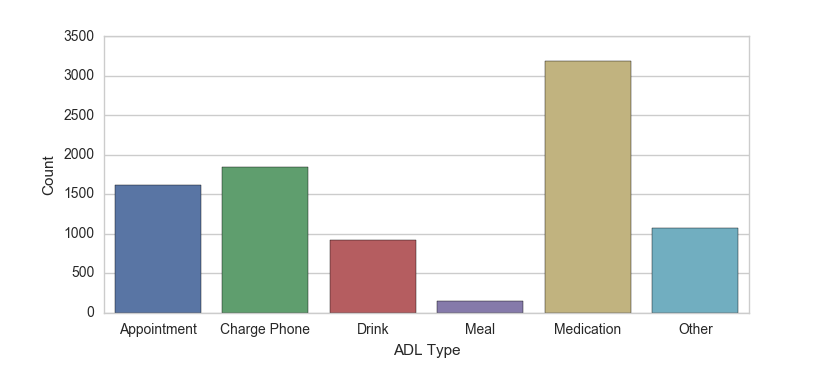
\includegraphics[scale=0.7, angle=0]{Files/treatment-study-1/figures/adl-type}
        \caption{Types of Acknowledged and Missed Reminders (n=8784) for DC participants.}
        \label{fig: adl-type}
\end{figure}


\section{Pre-Processing}
The proposed system should be able to regulate, through postponing or escalating, the delivery of reminders based on currently observed context states.
As such, the model will need to recognise the contexts which have had a historically high rate of acknowledgment, and those which have not. This can be performed via machine learning, by training a classifier, using each reminder's acknowledgement status as a class label.

To aid this step, the author developed a bespoke program\footnote{Source code available at: https://github.com/pjhartin/python-sensoranalysis-taut}, utilising the open source scientific tools provided in the \texttt{SciPy} and \texttt{NumPy} packages, to aid with the processing of the data generated within the app. The program was designed to pair, and label, the raw sensor data with the reminder data, validate the pairing, and facilitate the pre-processing, including filtering, windowing and feature extraction, of sensor data.

\subsection{Feature Selection}
Raw sensor data is varied and complex. It is, however, possible to derive a subset of values, or features, from the data which describe the data at a high level. Often these features are simple mathematical and statistical metrics, yet they describe the key characteristics of the signal.

Having demonstrated efficacy in all manner of classification problems \cite{Figo2010, Dargie2009, Bao2004}, the following 11 statistical features were calculated for each sensor recording in this study:

\begin{itemize}[noitemsep,topsep=0pt]
  \item Mean
  \item Median
  \item Minimum
  \item Max
  \item Variance
  \item Standard Deviation
  \item Root Mean Square
  \item Sum
  \item Range
  \item 75\% percentile cut-off
  \item 25\% percentile cut-off
\end{itemize}
% percentile cut offs?

In the example of accelerometer data, a 10 second sample, sampled at 100Hz, contains 10,000 values. A number of useful features can be selected from this sample, to describe the entire window of data. An example performed on two sample accelerometer signals is shown in Figure \ref{fig: feature-selection-example}. As such, it becomes very simple and efficient to compare multiple sensor recordings against one another based upon their features.

\begin{figure}[h]
    \centering
        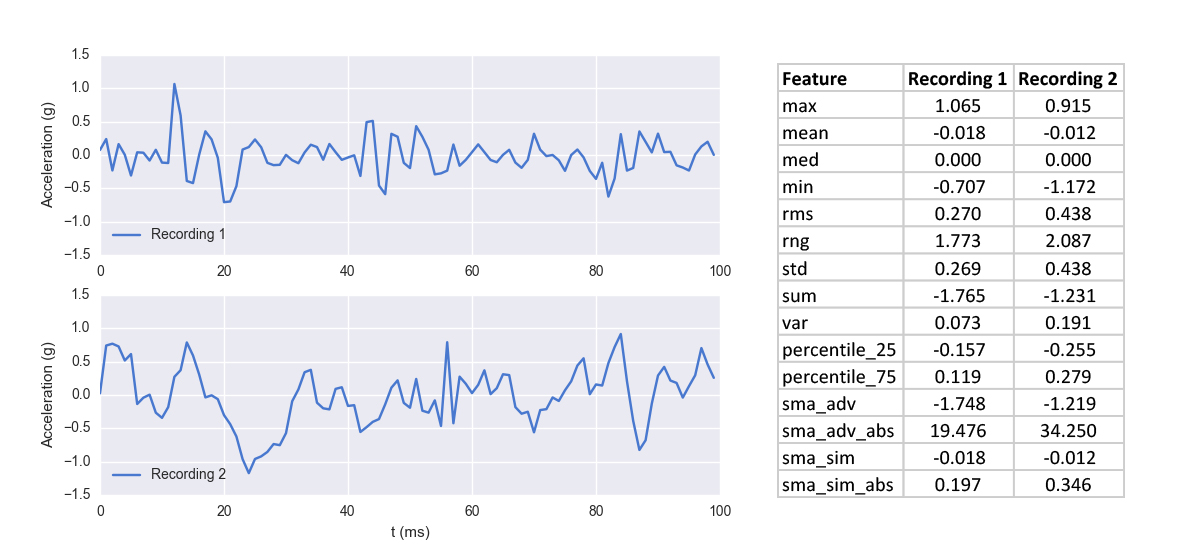
\includegraphics[scale=0.38, angle=0]{Files/treatment-study-1/figures/feature-selection-example}
        \caption{Example of feature selection performed on two similar accelerometer wave samples.}
        \label{fig: feature-selection-example}
\end{figure}

A key concept of the approach is that feature selection results in a set of relevant features, whilst removing redundant or irrelevant features which could negatively impact upon the accuracy of a classification model. The result is a set of features that are optimised to discriminate between the classes.
%VIVA: It is more that you are reducing the dimensionality of the problem as described by the feature vecore.  If this is reduced the classifier has an easier job at classifying the data.  The features assist in better discriminating between the classes.

\subsubsection{Signal Magnitude Area}
Multi-dimensional time-series data provides the opportunity to calculate additional features, such as the Signal Magnitude Area (SMA), as depicted in Equation \ref{eq: SMA},
\begin{equation}
SMA =\frac{1}{n} \left(\int_{0}^{n} \mid x(n)\mid \text{d} n + \int_{0}^{n} \mid y(n)\mid \text{d} n + \int_{0}^{n} \mid z(n)\mid \text{d} n  \right)
\label{eq: SMA}
\end{equation}
where $x$, $y$ and $z$ are the signals from each axis with respect to the sample number $n$, in a window.

The SMA has been used in studies as the basis to distinguish between periods of rest and activity \cite{Mathie2004, Karantonis2006}. The measure can be calculated in 2 ways:
\begin{description}
	\item [Simple] Calculated as simple sum of vector components, then normalised over length of the window.
	\item [Advanced] Calculated by subtracting the mean of the window from each of the axes to remove the average component
\end{description}

For thoroughness, both variations are calculated in this study when computing the SMA. In addition, the absolute values of both SMA variants are also recorded, resulting in 4 features per calculation.

\subsubsection{Frequency-Domain Analysis}
In similar works which aim to assess and quantify movement from accelerometers, frequency domain analysis has been used \cite{Preece2009}. The Fast Fourier Transform algorithm (FFT) \cite{Martens1992} has been frequently used in similar studies, after encouraging results were demonstrated by \citeauthor{Bao2004} for the classification of various movements in \citeyear{Bao2004} \cite{Bao2004}. The FFT transforms finite data, in this case windowed time-series data, into a spectrum of frequency components, showing their distribution. Additional features can be derived from the resulting data, by performing principal component analysis \cite{Preece2009} or extracting the energy spectrum \cite{Tapia2007}.
In previously published works by the author \cite{Hartin2014-WAGER}, the FFT algorithm was applied to windowed samples of both the accelerometer and the magnetometer signals. This application exposed limitations of the android platform for scientific application of FFTs. The android platform restricts a developer from explicitly setting a fixed sampling rate \cite{GoogleAndroid2016a}, resulting in inaccurate and incorrect frequency calculations. The cause is due to the variance in handset hardware. Since the Google Android platform cannot guarantee the hardware capabilities of each handset, the option to set the sampling rate (20Hz, 50Hz, 100Hz, etc.) or range (1.0g, 2.0g, 4.0g) is limited to choosing from a range of 4 options:

\begin{description}
	\item [\texttt{SENSOR\textunderscore DELAY\textunderscore UI}] suitable for the user interface
	\item [\texttt{SENSOR\textunderscore DELAY\textunderscore NORMAL}] suitable for screen orientation changes (default)
	\item [\texttt{SENSOR\textunderscore DELAY\textunderscore GAME}] suitable for games
	\item [\texttt{SENSOR\textunderscore DELAY\textunderscore FASTEST}] get sensor data as fast as possible
\end{description}

As such, in this study, the fastest option (\texttt{SENSOR\textunderscore DELAY\textunderscore FASTEST}) has been selected, which for the Motorola Moto G's hardware is 100Hz. This sampling rate, however, is still not guaranteed. The rate can vary due to processing and bandwidth bottlenecks on the device. As such, time to frequency transforms become computationally more expensive, especially on the device in real-time.

For these reasons, frequency domain features are not explored any further in this study.

\subsection{Summary of Features}
As the most promising features for the approach are yet to be established, the author employed a test-all approach, making use of all available features which have found successful application in other areas \cite{Figo2010}. In total, for each reminder instance, 330 features were calculated from the various sensors. These features are in-line with those typically used for context recognition from accelerometer data in similar studies \cite{Figo2010}.

\subsection{Processing Data Streams}
Although there are 4 sensors in the study, each sensor can provide a multitude of data streams, each of which can be processed further and used to create additional data sources. This sub-section will detail the data streams extracted from the sensors, and those created during processing.

\subsubsection{Multi-dimensional}
The accelerometer and magnetometer format their readings as a 4-dimensional array, consisting of time (t), and the 3-dimensions of space (x, y and z). Each individual dimension can be extracted from the array enabling a number of options for analysis. For example, it is possible to create a composite signal, by calculating the Signal Vector Magnitude (SVM) as described in Equation \ref{eq: SVM}.
\begin{equation}
SVM =\frac{1}{n} \sum_{i=1}^b \sqrt{x_i^2 + y_i^2 + z_i^2 }
\label{eq: SVM}
\end{equation}
where $x$, $y$ and $z$ are the signals from each axis with respect to the sample number $n$, in a window.

The SVM results in a single signal, which whilst losing a degree of fidelity, provides a good measure of the intensity of movement observed across all the axes \cite{Karantonis2006}. The SVM from accelerometry has been successfully utilised to classify various physical movements \cite{Gu2011,Banos2012,Pande2013}. In this study, the SVM is calculated for both the accelerometer and magnetometer signals, and used as an additional data source.


\subsubsection{Discrete Data}
The light and proximity sensors record their observations in a discrete manner in an effort to improve processing efficiency and battery life. When the sensor is first polled, a reading is taken. The sensor then polled at intervals checking for a change in value. If a value change is detected, the new value is recorded. This results in a 2 dimensional array, consisting of time and the observed value. An example of the discrete data imposed onto the continuous data observed from an accelerometer is presented in Table \ref{tbl: time-series-discretel}.

\begin{table}[h]
\centering
\caption{Example of continuous accelerometer series data and discrete sensor observations over time. Empty values for the discrete sensors assume the previously polled sensor value.}
\label{tbl: time-series-discretel}
\begin{tabular}{@{}ccccccc@{}}
\toprule
Time    & \multicolumn{4}{c}{Accelerometer} & Light        & Proximity    \\ \midrule
t    & x      & y      & z      & svm    & n            & n            \\ \midrule
1    & 1.245  & 0.569  & 10.042 & 4.772  & 65.12        & 5            \\
2    & 1.142  & 0.497  & 9.908  & 4.702  &              &              \\
3    & 1.218  & 0.511  & 9.810  & 4.704  &              &              \\
4    & 1.481  & 0.465  & 10.002 & 4.809  &              & 0            \\
5    & 1.285  & 0.566  & 9.832  & 4.738  &              &              \\
6    & 1.268  & 0.629  & 9.973  & 4.776  &              &              \\
7    & 1.299  & 0.624  & 10.015 & 4.792  &              & 5            \\
8    & 1.263  & 0.614  & 9.988  & 4.775  & 67.43        &              \\
9    & 1.315  & 0.533  & 10.041 & 4.783  &              &              \\
...  & ...    & ...    & ...    & ...    & ...          & ...          \\
t(i) & x(i)   & y(i)   & z(i)   & svm(i) & n(i) or last & n(i) or last \\ \bottomrule
\end{tabular}
\end{table}

\subsection{Filtering and Calibration}
Accelerometers and magnetometers found in smartphones are not designed to be high accuracy reference instruments. Often lower quality hardware is used, which results in noisy and uncalibrated signals \cite{Mitchell2013}. Despite this, smartphones are consistently used in scientific research due to their widespread prevalence and potential use cases. To counter the noise found in smartphone sensors, filtering is commonly applied to the signals.
%VIVA: Be prepared to discuss filtering during the VIVA!

\subsubsection{Filtering}
Having shown efficacy in similar studies \cite{Xia2011}, a median filter was chosen as an appropriate filter to remove noise from each signal. The median filter, when applied, transforms a list of values across a window length, based upon the median value for that window. The optimal size of the sliding-window depends upon the signal input and the desired level of smoothing.
To determine the appropriate size for this study, a number of tests were performed.

\textbf{Sliding Window-Length.}
Firstly a number of samples of missed and acknowledged reminders were chosen to study. For each recording the statistical features were extracted and recorded.
A range of window lengths (3-61) were then applied to the samples. From the resulting filtered signal, the same statistical features were calculated.
%VIVA: Why 3-61?
As the system aims to solve a binary classification problem (recognising acknowledged or missed), it was decided that the numerical difference between the features was key to a classifier's success. As such, a percentage difference comparison between the features of missed and acknowledged reminders was then performed for the raw and filtered data of various window lengths.
From the samples, the mean percentage difference between the classes (Acknowledged, Missed) for the unfiltered data, was 54\%, as seen in Figure \ref{fig: filter-percentage-difference} and Table \ref{tbl: percentage-difference-example}. Filtering the data using a median filter, with the minimum window length of 3 immediately improved the percentage difference observed. As presented in Figure \ref{fig: filter-percentage-difference}, increasing the window-length continues to widen the percentage difference in the features from the two classes.

\begin{figure}[]
    \centering
        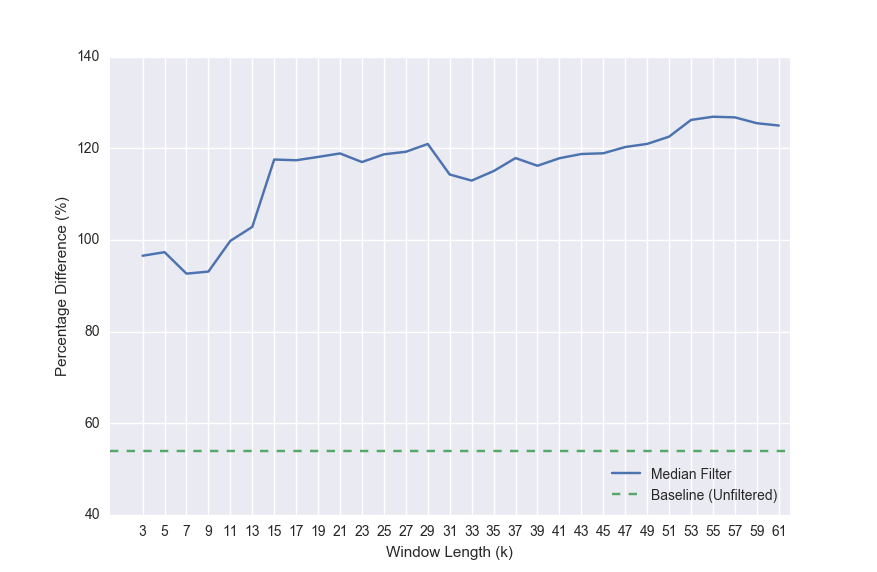
\includegraphics[scale=0.65, angle=0]{Files/treatment-study-1/figures/filter_window_length}
        \caption{Mean percentage difference observed between missed and acknowledged features for median filter window lengths.}
        \label{fig: filter-percentage-difference}
\end{figure}

At a window-length of 15, the difference reaches its first peak, after which, future improvement comes at computationally diminishing returns, eventually plateauing at the maximum of 61. An example of output from the process, using the observed optimal window-length of 15 for the median filter is shown in Table \ref{tbl: percentage-difference-example}.
%VIVA: Chris comment -  Has this been a subjective process if limited data has been used to define the window length.  I guess it is difficult to justify this either way.

\begin{table}[]
\centering
\caption{Comparison of extracted features and their percentage difference between classes in filtered and unfiltered data.}
\label{tbl: percentage-difference-example}
\resizebox{\textwidth}{!}{%
\begin{tabular}{@{}lllllll@{}}
 & \multicolumn{3}{c}{Raw (No Filter)} & \multicolumn{3}{c}{Median Filter (k=15)} \\ \midrule
Feature & Missed & Acknowledged & Difference (\%) & Missed & Acknowledged & Difference (\%) \\ \midrule
max & 31.4329 & 9.6185 & 106.28 & 0.2363 & 1.2724 & 137.35 \\
mean & 0.0610 & 0.0941 & 42.73 & 0.0052 & 0.0611 & 168.82 \\
min & -1.9669 & -3.0805 & 44.13 & -1.9682 & -0.5349 & 114.52 \\
percentile 25 & -0.1244 & -0.2036 & 48.32 & -0.0409 & -0.0912 & 76.13 \\
percentile\_75 & 0.1616 & 0.3051 & 61.47 & 0.0441 & 0.1988 & 127.34 \\
rms & 1.1788 & 0.7953 & 38.85 & 0.1065 & 0.2553 & 82.27 \\
rng & 33.3997 & 12.6991 & 89.81 & 2.2045 & 1.8073 & 19.80 \\
sma\_adv & 48.7090 & 75.1810 & 42.73 & 4.1303 & 48.8546 & 168.82 \\
sma\_adv\_abs & 232.7426 & 358.4968 & 42.54 & 50.1466 & 146.0025 & 97.74 \\
sma\_sim & 0.0610 & 0.0941 & 42.73 & 0.0052 & 0.0611 & 168.82 \\
sma\_sim\_abs & 0.2913 & 0.4487 & 42.54 & 0.0628 & 0.1827 & 97.74 \\
std & 1.1772 & 0.7897 & 39.40 & 0.1063 & 0.2478 & 79.90 \\
sum & 48.7700 & 75.2751 & 42.73 & 4.1354 & 48.9157 & 168.82 \\
var & 1.3858 & 0.6236 & 75.85 & 0.0113 & 0.0614 & 137.80 \\ \midrule
Mean & - & - & 54.29 & - & - & 117.56 \\ \bottomrule
\end{tabular}
}
\end{table}

The median filter with a window-length of 15 provides an inexpensive method of filtering a signal, and displays efficiency in removing outliers whilst retaining detail. An example of this can be found in Figure \ref{fig: apply-filter}, where a recording from the study displays noise and artificial spikes in the data.

\begin{figure}[h]
    \centering
        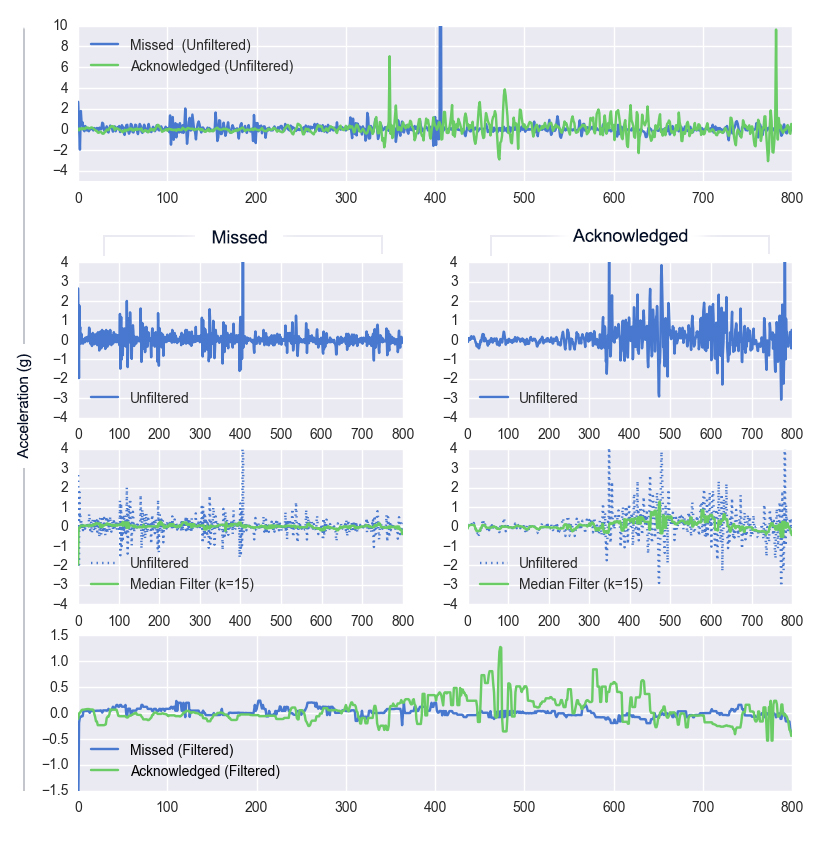
\includegraphics[scale=0.5, angle=0]{Files/treatment-study-1/figures/filtering_figure}
        \caption{Application of median filter (k=15) to accelerometer data. Resultant signal shows removal of noise, making the difference in each waveform more prominent.}
        \label{fig: apply-filter}
\end{figure}


\subsubsection{Calibration}
In addition to filtering, calibration was performed on the accelerometer and magnetometer data. Correctly performed, calibration enables all the recordings to have the same point of reference, resulting in precise, accurate and valid comparisons.
Whilst rudimentary calibration can be performed in the field \cite{Ferraris1995}, it requires a level of user input and knowledge which the author did not wish to ask of the end-users with dementia. The author also did not have any physical access to the handsets prior to deployment, and as a result, could not guarantee the devices were calibrated accurately.
Initial screening of the recorded data from various users uncovered that accelerometer readings were offset to various degrees depending on the device. Whilst this is a non-issue when comparing data from the same device as the offset is shared amongst all the recordings, the lack of calibration makes comparison with data observed from another device less valid.
To address this issue, for each SVM signal, the signal was reproduced, with an offset set as the median value of the signal. This rudimentary method resulted in a SVM which was effectively calibrated to 0, whilst maintaining the same shape and features, allowing much more accurate comparisons across devices.
%VIVA: Chris - Have you any references to support this approach?  I suspect this will be discussed at the viva
%VIVA: P - Whilst such an approach on live streaming data would be counter productive and drastically skew any data observed, having the entire of 6 minutes gave a large range of data from which to establish the true median value, or x-intercept.

\subsection{Windowing}
Although each sensor recording is 6 minutes in duration, the resulting system aims to \textit{predict} if a reminder will be acknowledged or missed. therefore only data observed before the reminder was delivered can be used.
The immediate point of reminder delivery is selected as the cutoff point in the signal, a figure which is extracted from the reminder log data, as illustrated in Figure \ref{fig: accelerometer-full-windowed}.

\begin{figure}[h]
    \centering
        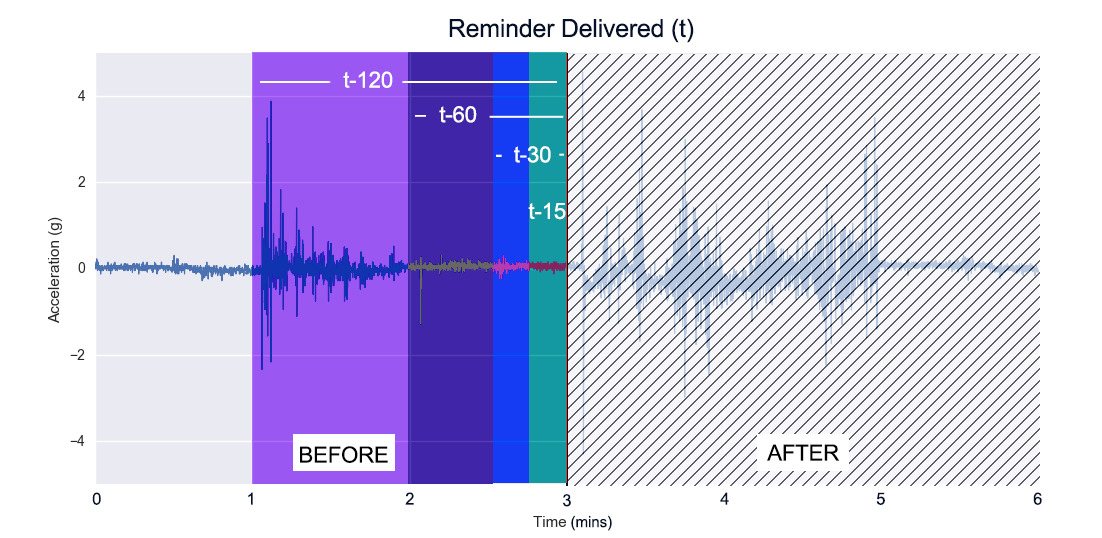
\includegraphics[scale=0.35, angle=0]{Files/treatment-study-1/figures/accelerometer-full-windowed}
        \caption{Illustration of signal windowing, with window endpoint as time of reminder delivery (t), and start point calculated by subtracting the desired window lengths (t-k).}
        \label{fig: accelerometer-full-windowed}
\end{figure}

The resulting signal is approximately 3 minutes long, and contains only the sensors readings \textit{prior} to the reminder being issued.
To establish an appropriate window length, a range of values were tested (10, 15, 20, 30 seconds). Whilst smaller windows, in the order of 1-5 seconds, have been shown to be useful in the recognition of different physical activities \cite{Wagenaar2011, Khan2014}, preliminary testing suggested that for this application, measurements extracted from larger windows provided greater distinguishing features. It is from these windows that the features were extracted.

\subsection{Labelling}
Using the acknowledgement data generated from each reminder delivery, it is possible to label each feature as acknowledged or missed for the purposes of training and validation within the supervised machine-learning phase.

\subsection{Classification}
Once all the features have been selected and labelled for their respective classes, the data is ready to be used to build a classifier. In this study, the Waikato Environment for Knowledge Analysis (Weka)  machine learning and experimentation suite \cite{Hornik2009} was used as the primary tool for the development of classification models. Weka provides a number of classification and modeling algorithms commonly used in context-aware applications, including:
\begin{description}[noitemsep,topsep=0pt]
	\item [J48] A C4.5 decision tree learner
	\item [NaiveBayes] A Naive Bayesian learner.
	\item [Logistic] Logistic Regression.
	\item [SMO] A Support Vector Machine (linear, polynomial and RBF kernel)
	\item [KStar] Instance-Based learner.
	\item [IBk] Instance-Based nearest neighbour learner with fixed neighbourhood.
	\item [JRip] A clone of the RIPPER rule learner.
\end{description}

As no single classifier family has had a distinct advantage in context or activity classification problems \cite{Mitchell2013a}, the author examined all possible options provided by the Weka tool. In each case, a classifier's performance is benchmarked against the ZeroR classifier, which predicts the modal, or majority, class for all future instances. E.g., for a data set of 60 instances of Class A, and 40 instances of Class B, the ZeroR classifier will classify all new instances as the most frequently occurring class (Class A), resulting in an baseline accuracy of 60\%.

\subsubsection{Measures of Comparison}
Accuracy, when used as the main metric of comparison can be a misleading representation of a classifiers performance. In addition to the accuracy (percentage correct), the sensitivity (precision), specificity (recall), Kappa statistic and the Area Under the ROC curve are also considered in the comparison of results.

\textbf{Sensitivity.}
The sensitivity, or precision, of a classifier is the proportion of instances that were truly of a class divided by the total instances classified as that class.

\textbf{Specificity.}
The specificity, or recall, of the classifier is the proportion of instances classified as a given class divided by the actual total in that class. This is also equivalent to True Positive rate.
%VIVA: Understand precision and recall?

\textbf{F-Measure.} The F-Measure is a combined measure for precision and recall, giving the mean for equally weighted measures.

\textbf{Kappa Statistic.}
The kappa statistic is a valuable measure to compare classifiers amongst themselves. The statistic is the result of the comparison between the observed accuracy of the classifier, with an expected accuracy, obtained through random chance. An advantage of using the kappa statistic to compare classifiers is the ability to categorise into performance groups, such as those proposed by \citeauthor{Landis1977}: 0-0.20 as slight, 0.21-0.40 as fair, 0.41-0.60 as moderate, 0.61-0.80 as substantial, and 0.81-1 as almost perfect \cite{Landis1977}.

\textbf{Area Under Curve (ROC).}
The Area Under Curve metric measures the performance of a binary classification. When used in a regression classification for a binary class problem, it is possible to plot the probability threshold changes in an ROC curve \cite{Metz1978}. This curve plots the True Positive rate against the False positive rate. An example ROC graph is presented in Figure \ref{fig: auc-roc-example}.

\begin{figure}[h]
    \centering
        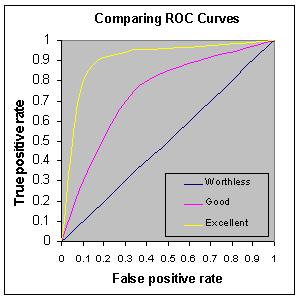
\includegraphics[scale=3, angle=0]{Files/treatment-study-1/figures/auc-roc-example}
        \caption{Illustration of Area Under an ROC including example ratings of model fit. Image Source: \fullcite{Tape} \cite{Tape}.}
        \label{fig: auc-roc-example}
\end{figure}

The graph essentially shows that given a random class A and class B observation, the area under the curve gives the proportion of correct guesses. The area under the ROC curve (AUC) is much less affected by the sample balance than the accuracy metric. To understand the rankings of the metric, a perfect model has an area of 1, whilst purely random is 0.5.
Medical practitioners using the AUC suggest the following classifications for the models fit \cite{Tape}:
\begin{itemize}[noitemsep,topsep=0pt]
  \item \textgreater .90 - Outstanding
  \item .80-.90 - Excellent (Good)
  \item .70-.80 - Acceptable (Fair)
  \item .60-.70 - Poor
  \item .50-.60 - No Discrimination
\end{itemize}

\subsection{Overview}
The order of the process is displayed in Figure \ref{fig: process-overview}. Raw sensor data is downloaded from the device, paired with reminder data, windowed, filtered, and features are extracted from both filtered and non-filtered data. The features are then appended to a list, and exported to external file system as both a labelled csv file, and a Weka formatted arff file.

\begin{figure}[h]
    \centering
        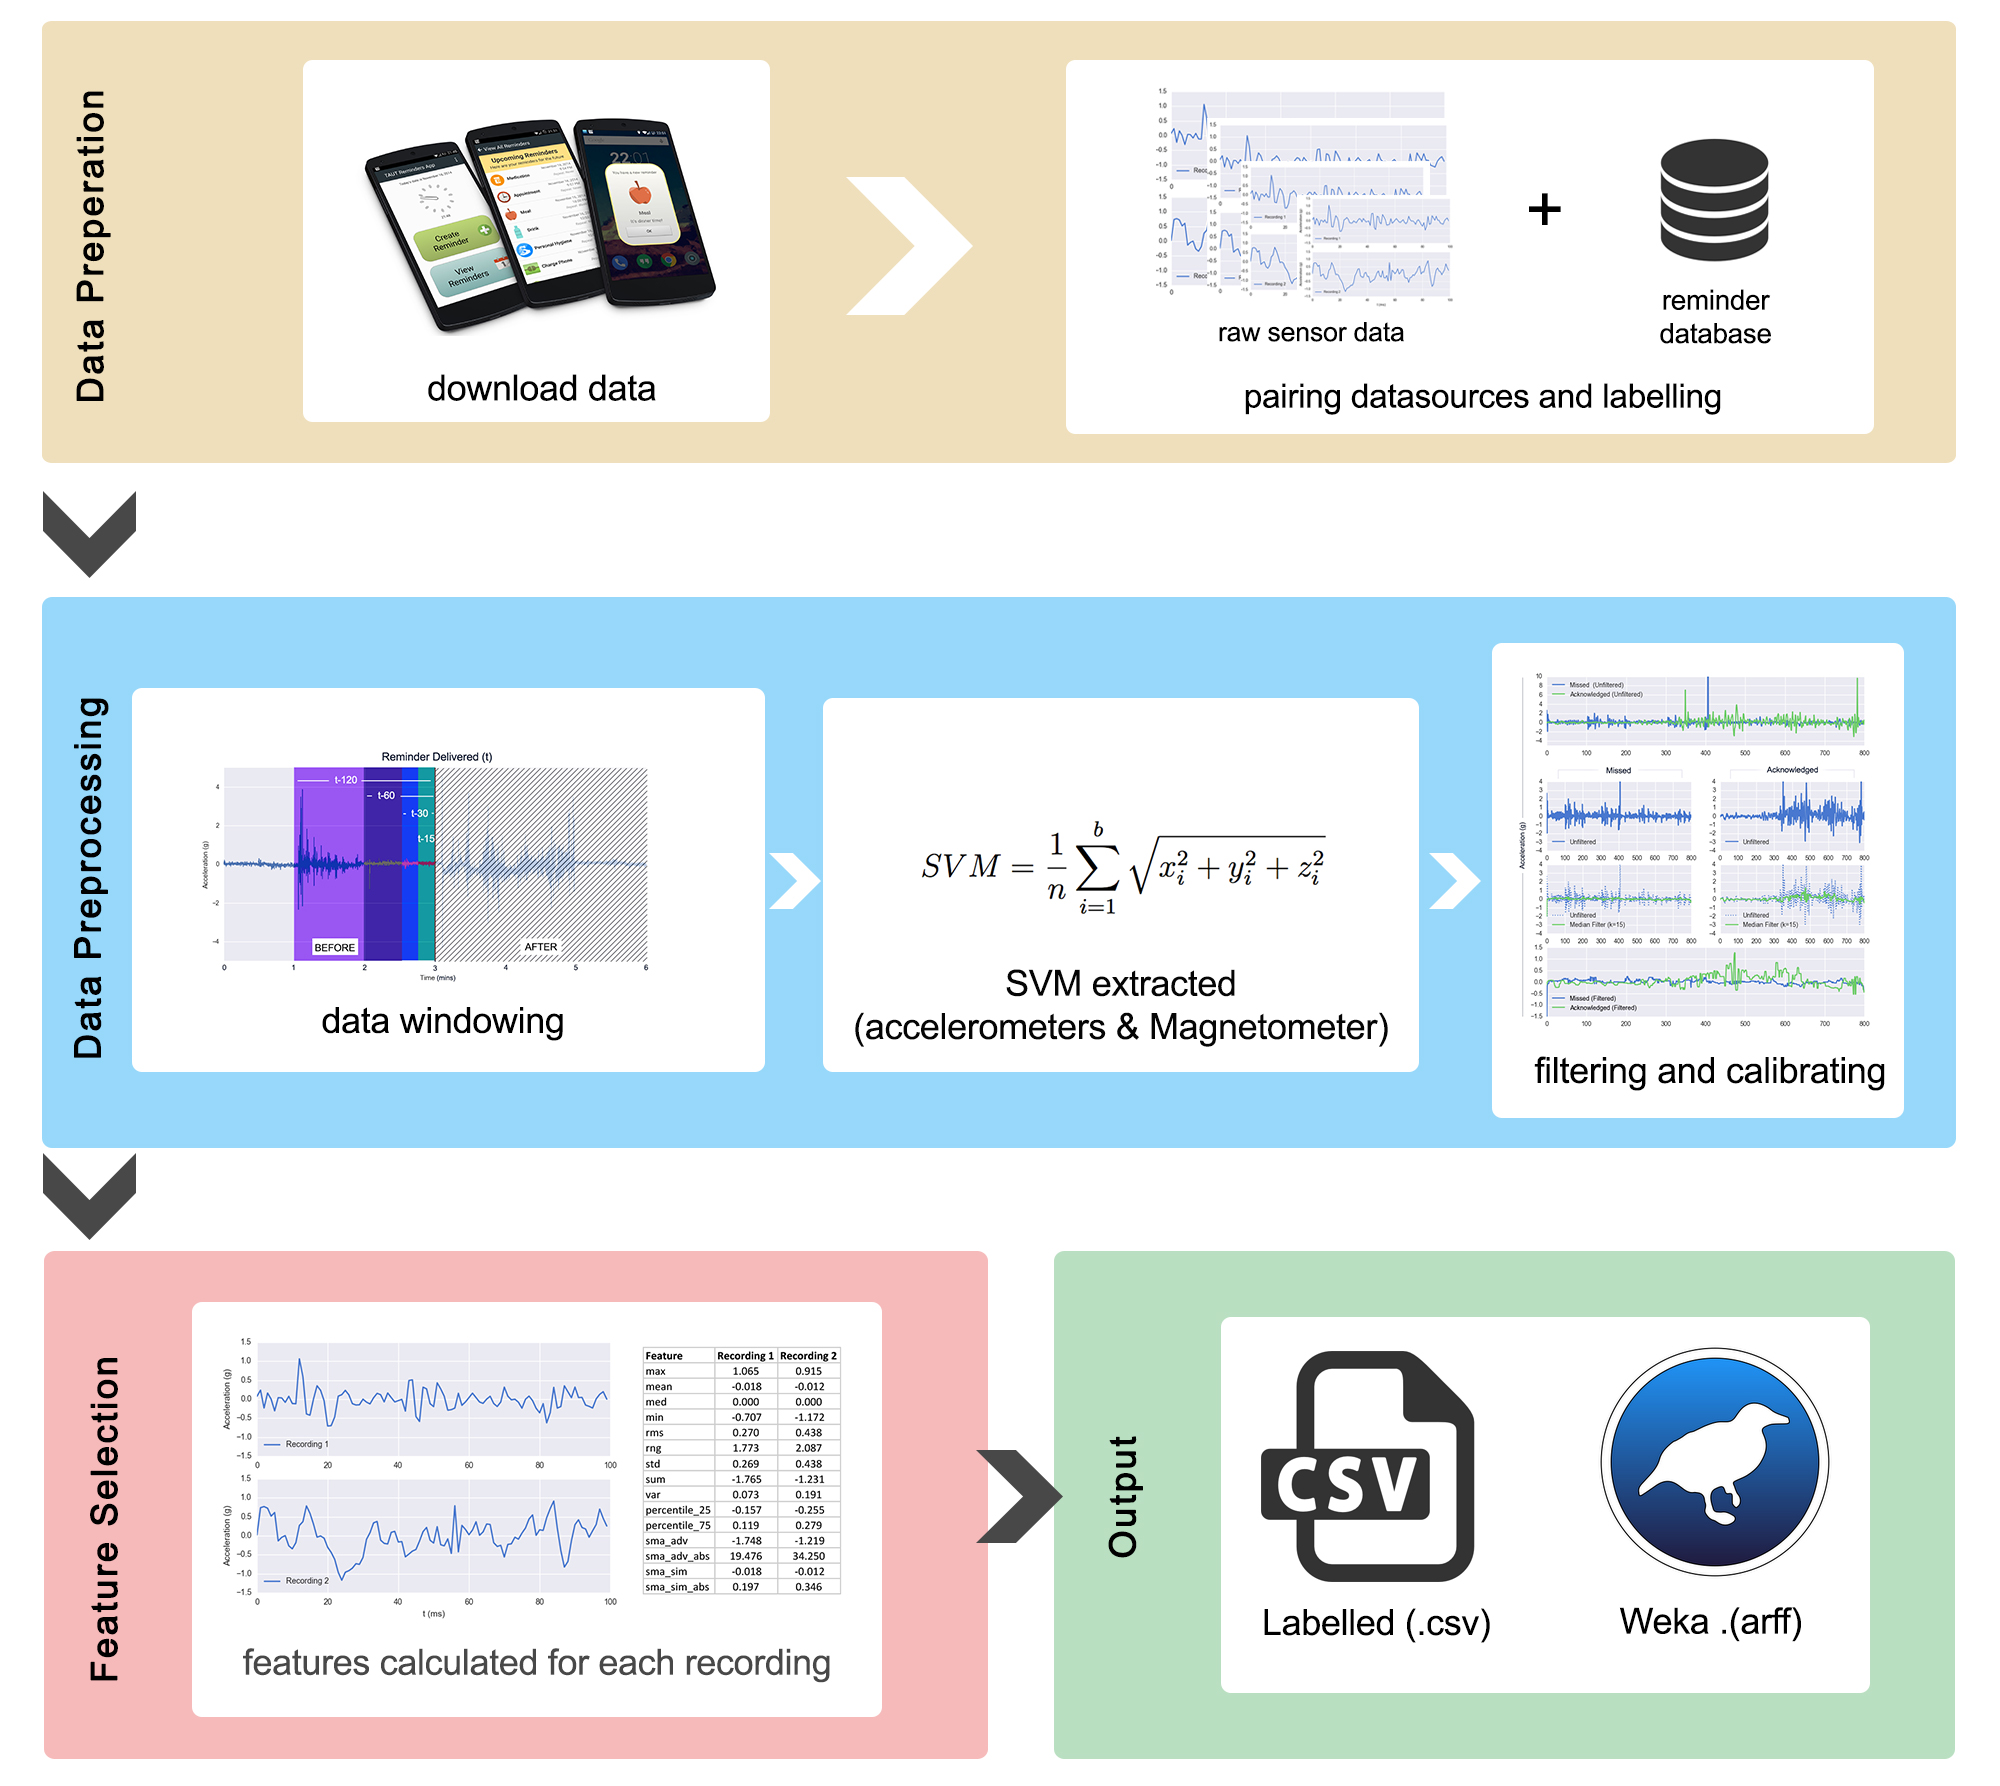
\includegraphics[scale=0.2, angle=0]{Files/treatment-study-1/figures/process-outlined}
        \caption{Illustration of procedure, from data collection, to pre-processing, feature selection, and output.}
        \label{fig: process-overview}
\end{figure}

\section{Results} \label{section: taut-results}
This Section details the results from the application of various classifiers to the resulting datasets of the TC and DC studies. In addition, the application of ensemble methods and data balancing are also explored, along with the evaluation of personalised models.

\subsection{Generalised Model}
Combining the data from all the participants in each study, respectively, resulted in 2 large datasets. These datasets were subsequently used in an effort to create a generalised model to predict missed or acknowledged reminder contexts. The data from the DC is explored first, and later contrasted to the TC data.

\subsubsection{Base Accuracy}
From the pre-processing stage a multitude of datasets were output for each window length (15, 20, 30, 45, 60, 90 seconds). Each dataset was analysed independently in an attempt to establish the optimal window length and classifier choice for future analysis. This was performed by applying a range of classifiers to the various windowed datasets. The results are presented in Table \ref{tbl: base-accuracy-windows}. Note that KStar (K*), an instance based-classifier, was removed from the analysis due to poor performance in the development of a generalised model in previous works by the author \cite{Hartin2014-WAGER}.

\begin{table}[h]
\centering
\caption{Accuracy (\%) of classifiers tested for numerous window lengths, showing statistically significant improvement and degradation over base ZeroR classifier at the p \textless .05 level.}
\label{tbl: base-accuracy-windows}
\resizebox{\textwidth}{!}{%
\begin{tabular}{@{}llllllllllllll@{}}
\toprule
\begin{tabular}[c]{@{}l@{}}Window\\ Size\end{tabular} & \begin{tabular}[c]{@{}l@{}}ZeroR\\ (Base)\end{tabular} & J48 &  & \begin{tabular}[c]{@{}l@{}}Naive \\ Bayes\end{tabular} &  & Logistic &  & SMO &  & IBK &  & JRip &  \\ \midrule
15s & 72.84 & 80.31 & $\circ$ & 53.17 & $\bullet$ & 78.26 & $\circ$ & 76.27 & $\circ$ & 51.24 & $\bullet$ & 81.14 & $\circ$ \\
20s & 72.84 & 81.23 & $\circ$ & 51.56 & $\bullet$ & 78.86 & $\circ$ & 76.47 & $\circ$ & 55.62 & $\bullet$ & 81.60 & $\circ$ \\
30s & 72.84 & 79.93 & $\circ$ & 52.19 & $\bullet$ & 79.27 & $\circ$ & 76.38 & $\circ$ & 54.61 & $\bullet$ & 81.83 & $\circ$ \\
45s & 72.84 & 79.64 & $\circ$ & 52.05 & $\bullet$ & 79.67 & $\circ$ & 76.47 & $\circ$ & 57.09 & $\bullet$ & 81.75 & $\circ$ \\
60s & 72.84 & 81.29 & $\circ$ & 52.11 & $\bullet$ & 79.30 & $\circ$ & 76.50 & $\circ$ & 56.92 & $\bullet$ & 81.57 & $\circ$ \\
90s & 72.84 & 79.70 & $\circ$ & 52.22 & $\bullet$ & 78.95 & $\circ$ & 76.38 & $\circ$ & 55.97 & $\bullet$ & 81.66 & $\circ$ \\ \midrule
\multicolumn{14}{c}{$\circ$, $\bullet$ statistically significant improvement or degradation at the p\textless .05 level} \\ \bottomrule
\end{tabular}
}
\end{table}

Looking at rest of data, decision tree and rule-based classifiers, J48 and JRip, are performing the best. A window size of 30s provided the best performance for JRip, whilst 20s was best for J48. Analysis of the other comparison measures between these window sizes can be found in Table \ref{fig: window-length-measure-comparison}.

\begin{table}[h]
\centering
\caption{Comparison of classification performance measures for 20 and 30 second window lengths.}
\label{fig: window-length-measure-comparison}
\resizebox{\textwidth}{!}{%
\begin{tabular}{@{}llllllllll@{}}
\toprule
Measure & \begin{tabular}[c]{@{}l@{}}Window\\ Length\end{tabular} & \begin{tabular}[c]{@{}l@{}}ZeroR \\ (Base)\end{tabular} & J48 & \begin{tabular}[c]{@{}l@{}}Naive \\ Bayes\end{tabular} & Logistic & SMO & IBk & JRip & Mean \\ \midrule
\multirow{2}{*}{Precision} & 20 & 0 & 0.66 & 0.34 & 0.66 & 0.8 & 0.35 & 0.68 & 0.58 \\
 & 30 & 0 & 0.63 & 0.35 & 0.66 & 0.77 & 0.35 & 0.68 & 0.57 \\ \midrule
\multirow{2}{*}{Recall} & 20 & 0 & 0.64 & 0.86 & 0.46 & 0.18 & 0.71 & 0.61 & 0.58 \\
 & 30 & 0 & 0.63 & 0.89 & 0.48 & 0.19 & 0.75 & 0.64 & 0.60 \\ \midrule
\multirow{2}{*}{F-Measure} & 20 & 0 & 0.65 & 0.49 & 0.54 & 0.29 & 0.47 & 0.64 & 0.51 \\
 & 30 & 0 & 0.63 & 0.5 & 0.56 & 0.3 & 0.47 & 0.65 & 0.52 \\ \midrule
\multirow{2}{*}{Kappa} & 20 & 0 & 0.52 & 0.16 & 0.41 & 0.22 & 0.16 & 0.52 & 0.33 \\
 & 30 & 0 & 0.49 & 0.18 & 0.43 & 0.22 & 0.16 & 0.53 & 0.34 \\ \midrule
\multirow{2}{*}{ROC} & 20 & 0.5 & 0.78 & 0.64 & 0.79 & 0.58 & 0.61 & 0.76 & 0.69 \\
 & 30 & 0.5 & 0.77 & 0.64 & 0.8 & 0.58 & 0.61 & 0.77 & 0.70 \\ \bottomrule
\end{tabular}
}
\end{table}

From the Table, it is clear that the differences between the two window sizes are extremely small. In all measures, with the exception of precision, the 30 second window size performs marginally better. As such, all future analysis was performed on the data derived from the 30 second window.

\subsubsection{Ensemble Methods}
Whilst the J48 (79.93\%) and JRip (81.83\%) classifiers were performing statistically significantly better than a majority classifier (72.84\%), there are still a number of ways in which to further boost the performance of the models. Identified as one of the top 10 algorithms in data mining by \citeauthor{Wu2007} \cite{Wu2007}, ensemble methods such as boosting, bagging and blending (or stacking) can improve classification performance in a myriad of tasks, and are especially useful when dealing with C4.5 decision trees (J48).

\textbf{Boosting.}
Boosting uses a base classifier to build a model based upon the training data, after which, a second classifier is then created to focus on the instances that the first classifier predicted incorrectly. The process continues until a limit of models or accuracy is achieved.

\textbf{Bagging.}
Bagging creates separate training samples from the original dataset, and creates a classifier for each sample. Through averaged or majority voting the results of the classifiers are combined to create a base classifier. This methods strength is based on the premise that the separate training samples have subtly unique perspectives on the classification problem. 

\textbf{Blending.}
Blending, or stacking, involves using multiple different classification algorithms to prepare a model on the training data. After which, a combiner algorithm, or meta-classifier, is trained to make the final prediction, using the predictions of the other classifiers as inputs.

As the J48 and JRip algorithms performed best on the data in the previous section, J48 was used as the base classifier for both boosting and Bagging, and a combination of J48 and JRip were used for the Blending (Stacking) algorithm. Each was applied to the DC's data, and the results compared against the J48 (C4.5 decision tree) from the previous section. Full results are displayed in Table \ref{tbl: utah-ensemble-results}. The application of Bagging (J48) and Blending (J48 with JRip) resulted in significant improvement in accuracy, precision and ROC over the base J48, whilst significantly decreasing recall. In this case, the decrease in recall (True Positive Rate) is the ability to correctly identify a context in which acknowledgements occurred. An ROC of over .8, as found with the ensemble methods would be considered an excellent fit by the guidelines outlined in \cite{Tape}.

\begin{table}[h]
\centering
\caption{Results of ensemble classifiers applied to DC dataset, showing statistical significance against J48 (C4.5 Decision Tree) as base comparison.}
\label{tbl: utah-ensemble-results}
\resizebox{\textwidth}{!}{%
\begin{tabular}{@{}llllllllllll@{}}
\toprule
Measure & \begin{tabular}[c]{@{}l@{}}J48 \\ (Base)\end{tabular} & ZeroR &  & JRip &  & \begin{tabular}[c]{@{}l@{}}Boosting \\ (J48)\end{tabular} &  & \begin{tabular}[c]{@{}l@{}}Bagging \\ (J48)\end{tabular} &  & \begin{tabular}[c]{@{}l@{}}Blending \\ (J48/JRip)\end{tabular} &  \\ \midrule
Accuracy (\%) & 79.93 & 72.84 & $\bullet$ & 81.83 &  & 78.69 &  & 81.89 & $\circ$ & 81.92 & $\circ$ \\
Precision & 0.63 & 0 & $\bullet$ & 0.68 & $\circ$ & 0.62 &  & 0.71 & $\circ$ & 0.71 & $\circ$ \\
Recall & 0.63 & 0 & $\bullet$ & 0.64 &  & 0.57 & $\bullet$ & 0.57 & $\bullet$ & 0.56 & $\bullet$ \\
F-Measure & 0.63 & 0 & $\bullet$ & 0.65 &  & 0.59 & $\bullet$ & 0.63 &  & 0.62 &  \\
Kappa & 0.49 & 0 & $\bullet$ & 0.53 &  & 0.45 &  & 0.51 &  & 0.51 &  \\
ROC & 0.77 & 0.5 & $\bullet$ & 0.77 &  & 0.82 & $\circ$ & 0.85 & $\circ$ & 0.82 & $\circ$ \\ \midrule
\multicolumn{12}{c}{$\circ$, $\bullet$ statistically significant improvement or degradation at the p\textless .05 level} \\ \bottomrule
\end{tabular}
}
\end{table}

\subsubsection{Balancing the Dataset}
Whilst the ensemble methods did improve the classification performance, it was apparent that the classes (Acknowledged/Missed) were not represented equally in the data, and as such any model built upon the training data will be imbalanced to the majority class. Imbalance in datasets is common, and in this case, was expected. The ratio of Missed (n=2562) to Acknowledged (n=942) reminders is almost 35:13 (421:157 Simplified). To balance the training dataset to 50:50 (Kappa = 0) a number of methods may be used which may be referred to as stratification.

\textbf{Resampling.}
Resampling is performed by simply replicating instances of the minority class back into the training set until the distribution is equal. 

\textbf{Downsampling.}
Downsampling is the opposite approach, and involves removing instances from the majority class, so that the distribution is equal. 

Both of these methods bring distinct disadvantages, namely overfitting to the minority class in resampling, and losing truth and variance in downsampling. An ideal and optimal approach is the use of synthetic data \cite{nonnemaker2008}.

\textbf{Synthetic Data.} The generation of synthetic data based on the minority class is a method of balancing the dataset. The most popular of such algorithms is the Synthetic Minority Over-sampling Technique (SMOTE). SMOTE functions by selecting a number of instances, and randomly alters the data one attribute at a time within a neighbouring difference of the selected instances. This results in the creation of additional instances that are similar, through statistical methods, however, not exact copies of instances from the same class \cite{Chawla2011}. SMOTE has been applied to many binary classification problems to help balance datasets across various research fields including pharmacology \cite{Kumari2015}, oncology \cite{Fehr2015}, information science \cite{Cleland2014-IWAAL, Zhang2013}, and even radar ornithology \cite{D.Rosa2016}.

Having applied SMOTE to the minority class (Acknowledged) to an effect of 168.16\%, resulted in a balanced dataset of 2526:2526 reminders.  
The same classifiers and ensemble methods were applied to the balanced dataset. Again, the basic J48 was used as the base of comparison for statistical significance tests between the classifiers as shown in Table \ref{tbl: utah-smote-classifiers}. In addition, comparisons between the datasets measures was also performed, as presented in Table \ref{tbl: utah-smote-dataset}.

\begin{table}[h]
\centering
\caption{Comparison of classifier performances on unbalanced dataset and SMOTE balanced dataset.}
\label{tbl: utah-smote-classifiers}
\resizebox{\textwidth}{!}{%
\begin{tabular}{@{}lllllllllllll@{}}
\toprule
Measure & Dataset & \begin{tabular}[c]{@{}l@{}}J48 \\ (Base)\end{tabular} & ZeroR &  & JRip &  & \begin{tabular}[c]{@{}l@{}}Boosting\\ (J48)\end{tabular} &  & \begin{tabular}[c]{@{}l@{}}Bagging\\ (J48)\end{tabular} &  & \begin{tabular}[c]{@{}l@{}}Blending \\ (J48/JRip)\end{tabular} &  \\ \midrule
\multirow{2}{*}{Accuracy (\%)} & Imbalanced & 79.93 & 72.84 & $\bullet$ & 81.83 &  & 78.69 &  & 81.89 & $\circ$ & 81.92 & $\circ$ \\
 & SMOTE & 78.31 & 50 & $\bullet$ & 80.07 &  & 82.98 & $\circ$ & 79.83 &  & 79.57 &  \\ \midrule
\multirow{2}{*}{F-Measure} & Imbalanced & 0.63 & 0 & $\bullet$ & 0.65 &  & 0.59 & $\bullet$ & 0.63 &  & 0.62 &  \\
 & SMOTE & 0.77 & 0 & $\bullet$ & 0.78 &  & 0.83 & $\circ$ & 0.78 &  & 0.79 &  \\ \midrule
\multirow{2}{*}{Kappa} & Imbalanced & 0.49 & 0 & $\bullet$ & 0.53 &  & 0.45 &  & 0.51 &  & 0.51 &  \\
 & SMOTE & 0.57 & 0 & $\bullet$ & 0.6 &  & 0.66 & $\circ$ & 0.6 &  & 0.59 &  \\ \midrule
\multirow{2}{*}{Precision} & Imbalanced & 0.63 & 0 & $\bullet$ & 0.68 & $\circ$ & 0.62 &  & 0.71 & $\circ$ & 0.71 & $\circ$ \\
 & SMOTE & 0.82 & 0 & $\bullet$ & 0.84 &  & 0.81 &  & 0.84 & $\circ$ & 0.82 &  \\ \midrule
\multirow{2}{*}{Recall} & Imbalanced & 0.63 & 0 & $\bullet$ & 0.64 &  & 0.57 & $\bullet$ & 0.57 & $\bullet$ & 0.56 & $\bullet$ \\
 & SMOTE & 0.73 & 0 &  & 0.74 &  & 0.86 & $\circ$ & 0.74 &  & 0.76 &  \\ \midrule
\multirow{2}{*}{ROC} & Imbalanced & 0.77 & 0.5 & $\bullet$ & 0.77 &  & 0.82 & $\circ$ & 0.85 & $\circ$ & 0.82 & $\circ$ \\
 & SMOTE & 0.85 & 0.5 & $\bullet$ & 0.82 &  & 0.9 & $\circ$ & 0.91 & $\circ$ & 0.89 & $\circ$ \\ \midrule
 \multicolumn{13}{c}{$\circ$, $\bullet$ statistically significant improvement or degradation at the p \textless .05 level} \\ \bottomrule
\end{tabular}
}
\end{table}

\begin{table}[ph]
\centering
\caption{Comparison of measures between unbalanced and balanced (SMOTE) DC dataset.}
\label{tbl: utah-smote-dataset}
\begin{tabular}{@{}lllll@{}}
\toprule
Measure                    & Classifier          & \begin{tabular}[c]{@{}l@{}}Utah \\ (Original)\end{tabular}  & \begin{tabular}[c]{@{}l@{}}Utah \\ (SMOTE)\end{tabular} &         \\ \midrule
\multirow{6}{*}{Accuracy (\%)}  & JRip                & 81.83 & 80.07                                                   &         \\
                           & J48                 & 79.93 & 78.31                                                   &         \\
                           & Boosting (J48)      & 78.69 & 82.98                                                   & $\circ$ \\
                           & Bagging  (J48)      & 81.89 & 79.83                                                   &         \\
                           & Blending (J48/JRip) & 81.92 & 79.57                                                   &         \\
                           & Average             & 79.52 & 75.11                                                   &         \\ \midrule
\multirow{6}{*}{Precision} & JRip                & 0.68  & 0.84                                                    & $\circ$ \\
                           & J48                 & 0.63  & 0.82                                                    & $\circ$ \\
                           & Boosting (J48)      & 0.62  & 0.81                                                    & $\circ$ \\
                           & Bagging  (J48)      & 0.71  & 0.84                                                    & $\circ$ \\
                           & Blending (J48/JRip) & 0.71  & 0.82                                                    & $\circ$ \\
                           & Average             & 0.56  & 0.74                                                    &         \\ \midrule
\multirow{6}{*}{Recall}    & JRip                & 0.64  & 0.74                                                    &         \\
                           & J48                 & 0.63  & 0.73                                                    &         \\
                           & Boosting (J48)      & 0.57  & 0.86                                                    & $\circ$ \\
                           & Bagging  (J48)      & 0.57  & 0.74                                                    & $\circ$ \\
                           & Blending (J48/JRip) & 0.56  & 0.76                                                    & $\circ$ \\
                           & Average             & 0.49  & 0.74                                                    &         \\ \midrule
\multirow{6}{*}{F-Measure} & JRip                & 0.65  & 0.78                                                    & $\circ$ \\
                           & J48                 & 0.63  & 0.77                                                    & $\circ$ \\
                           & Boosting (J48)      & 0.59  & 0.83                                                    & $\circ$ \\
                           & Bagging  (J48)      & 0.63  & 0.78                                                    & $\circ$ \\
                           & Blending (J48/JRip) & 0.62  & 0.79                                                    & $\circ$ \\
                           & Average             & 0.52  & 0.72                                                    &         \\ \midrule
\multirow{6}{*}{Kappa}     & JRip                & 0.53  & 0.6                                                     &         \\
                           & J48                 & 0.49  & 0.57                                                    &         \\
                           & Boosting (J48)      & 0.45  & 0.66                                                    & $\circ$ \\
                           & Bagging  (J48)      & 0.51  & 0.6                                                     &         \\
                           & Blending (J48/JRip) & 0.51  & 0.59                                                    & $\circ$ \\
                           & Average             & 0.42  & 0.5                                                     &         \\ \midrule
\multirow{6}{*}{ROC}       & JRip                & 0.77  & 0.82                                                    & $\circ$ \\
                           & J48                 & 0.77  & 0.85                                                    & $\circ$ \\
                           & Boosting (J48)      & 0.82  & 0.9                                                     & $\circ$ \\
                           & Bagging  (J48)      & 0.85  & 0.91                                                    & $\circ$ \\
                           & Blending (J48/JRip) & 0.82  & 0.89                                                    & $\circ$ \\
                           & Average             & 0.75  & 0.81                                                    &         \\ \midrule
\multicolumn{5}{c}{$\circ$, $\bullet$ statistically significant improvement or degradation at the p \textless .05 level} \\ \bottomrule
\end{tabular}
\end{table}

The application of the SMOTE algorithm resulted in an improvement in almost every measurement for each classifier. The best improvements can be found in the recall and ROC of the boosting, bagging and blending ensemble methods. Recall, a previous weak point of the system has now been improved substantially, resulting in an ROC of .91 (outstanding) in the bagging method.

\subsubsection{Feature Evaluation}
Whilst the classifier was generated using a dataset which contained 330 features, it is highly likely that only a limited number of these were used. It is possible to rank the importance of these features in the classifier, exposing features which have been calculated, yet are redundant to the model. Identifying these features and removing them, will optimise the speed at which features are calculated for the model, an important step if the features are to be eventually calculated on the device.

Using a forward traversing, greedy, best first search algorithm, and evaluation performed on a 5-fold J48 decision tree, the 330 features were reduced to 8 by the Weka software package:
\begin{description}[noitemsep,topsep=0pt]
	\item [accelerometer\textunderscore y\textunderscore rng] Range observed in the acceleration on the Y axis
	\item [accelerometer\textunderscore z\textunderscore median \textunderscore filter \textunderscore med] Median value of the accelerometer's filtered Z axis
	\item [light\textunderscore measure\textunderscore min] Minimum value observed from the light sensor
	\item [magnetic\textunderscore x\textunderscore median\textunderscore filter\textunderscore std] Standard deviation of the magnetometers filtered X axis
	\item [magnetic\textunderscore y\textunderscore median\textunderscore filter\textunderscore percentile\textunderscore 25] Cutoff of the 25th percentile of the magnetometers filtered Y axis
	\item [magnetic\textunderscore y\textunderscore median\textunderscore filter\textunderscore std] Standard deviation of magnetometer's filtered Y Axis
	\item [magnetic\textunderscore y\textunderscore percentile\textunderscore 25] Cutoff of the 25th percentile of the magnetometers raw Y axis
	\item [proximity\textunderscore measure\textunderscore min] Minimum observed value of the proximity sensor
\end{description}

As presented in Table \ref{tbl: utah-8-features}, whilst using only 8 features, the accuracy of the results improved substantially for the all classifiers on the unbalanced dataset (Original statistics in Table \ref{tbl: utah-ensemble-results}), whilst simultaneously reducing the build time from 99 seconds to 0.08 seconds. Note the 8 features still span all four sensor modalities provided by the smartphone. 

\begin{table}[h]
\centering
\caption{Statistics for classifiers trained and tested using reduced feature set (n=8), established through J48 evaluated Best First search. Dataset was original unbalanced.}
\label{tbl: utah-8-features}
\begin{tabular}{@{}lllllll@{}}
\toprule
Measure   & \begin{tabular}[c]{@{}l@{}}ZeroR \\ (Base)\end{tabular} & Jrip  & J48  & \begin{tabular}[c]{@{}l@{}}Boosting \\ (AdaBoost - J48)\end{tabular} & \begin{tabular}[c]{@{}l@{}}Bagging \\ (J48)\end{tabular} & \begin{tabular}[c]{@{}l@{}}Blending \\ (J48/JRip)\end{tabular} \\ \midrule
Accuracy (\%)  & 72.84                                                   & 83.13 & 83.1 & 80.39                                                                & 83.62                                                    & 83.04                                                          \\
Precision & 0                                                       & 0.7   & 0.71 & 0.65                                                                 & 0.73                                                     & 0.72                                                           \\
Recall    & 0                                                       & 0.67  & 0.63 & 0.6                                                                  & 0.62                                                     & 0.61                                                           \\
F-Measure & 0                                                       & 0.68  & 0.67 & 0.62                                                                 & 0.67                                                     & 0.66                                                           \\
Kappa     & 0                                                       & 0.57  & 0.56 & 0.49                                                                 & 0.56                                                     & 0.55                                                           \\
ROC       & 0.5                                                     & 0.79  & 0.82 & 0.83                                                                 & 0.85                                                     & 0.83                                                           \\ \bottomrule
\end{tabular}
\end{table}

\subsection{Comparison with Preliminary}
Whilst the results are promising with the data gathered from the DC, it is worthwhile to compare with the data gathered from the TC, described earlier in the Chapter. The TC cohort had a very different ratio of acknowledged to missed reminders, 90:16 (Acknowledged: Missed). To ensure fair comparison the same method of oversampling using SMOTE and applying ensemble classifiers was applied to the TC's dataset. SMOTE was applied to the minority case, which in the TC was the missed reminder class, to the effect of 462.5\%. The results from each ensemble method were compared between the DC(SMOTE) and TC(SMOTE) datasets and the results are shown in Table \ref{tbl: smote-compare-dc-tc}. No significant differences were found in the results of either dataset, suggesting that the generalised approach is a good method for both cohorts. In addition the ROC model fit classification for the DC and TC averaged at Outstanding (.9) and Excellent (.83), respectively. In the interest of fully exploring the data, the DC dataset (n = 3469) was used as the training set, and tested on the TC dataset (n = 106) using the strongest performing classifier tested in the study (Bagging using J48). The training and testing split in this case was 96.5\%:3.5\% (5052:180).
The resulting accuracy of the model was only 66\% (F-Measure 0.651), showing that each cohorts data were not applicable as a training sources for the other.

\begin{table}[h]
\centering
\caption{Comparison of ensemble method results for each measure when applied to SMOTE balanced datasets from DC and TC.}
\label{tbl: smote-compare-dc-tc}
\begin{tabular}{@{}llll@{}}
\toprule
Measure                    & Classifier & DC & TC \\ \midrule
\multirow{5}{*}{Accuracy (\%)}  & ZeroR      & 50                  & 50                    \\
                           & Boosting   & 82.98               & 76.67                 \\
                           & Bagging    & 79.83               & 77.78                 \\
                           & Blending   & 79.57               & 77.78                 \\
                           & Average    & 80.79               & 77.41                 \\ \midrule
\multirow{4}{*}{Precision} & Boosting   & 0.81                & 0.8                   \\
                           & Bagging    & 0.84                & 0.88                  \\
                           & Blending   & 0.82                & 0.82                  \\
                           & Average    & 0.82                & 0.83                  \\ \midrule
\multirow{4}{*}{Recall}    & Boosting   & 0.86                & 0.71                  \\
                           & Bagging    & 0.74                & 0.68                  \\
                           & Blending   & 0.76                & 0.72                  \\
                           & Average    & 0.79                & 0.70                  \\ \midrule
\multirow{4}{*}{F-Measure} & Boosting   & 0.83                & 0.74                  \\
                           & Bagging    & 0.78                & 0.74                  \\
                           & Blending   & 0.79                & 0.76                  \\
                           & Average    & 0.80                & 0.75                  \\ \midrule
\multirow{4}{*}{Kappa}     & Boosting   & 0.66                & 0.53                  \\
                           & Bagging    & 0.6                 & 0.56                  \\
                           & Blending   & 0.59                & 0.56                  \\
                           & Average    & 0.62                & 0.55                  \\ \midrule
\multirow{4}{*}{ROC}       & Boosting   & 0.9                 & 0.83                  \\
                           & Bagging    & 0.91                & 0.86                  \\
                           & Blending   & 0.89                & 0.81                  \\
                           & Average    & 0.90                & 0.83                  \\ \bottomrule
\end{tabular}
\end{table}


\subsection{Individual Model}
Whilst using a generalised model would help alleviate the cold start problem, the apparent variance between participants from both DC and TC suggested that an individualised model may yield superior results. To test this notion, each participant's data was filtered into their own dataset and tested against the configuration of classifiers identified in the generalised model section.

\subsubsection{Imbalanced Data}
Again the common issue of imbalanced data occurs, although more frequently in the analysis of the individual data. As the participants from the TC used the device for only 1 week, the total number of instances for this cohort is considerably lower. 
For many of the participants in both the DC and TC, it was not possible to perform 10-fold cross validation due to a lack of reminder instances. It was also not possible to use an 80:20 training testing split, as the ensemble methods still require a number of iterations to refine their supporting second or meta classifiers.

\subsubsection{Results}
For the participants for whom it was applicable, their data set was balanced through application of SMOTE.  J48 and Bagging with J48 classifiers were applied to each participant, and subsequently benchmarked against ZeroR as presented in Table \ref{tbl: smote-individual}.

\begin{table}[h]
\centering
\caption{Classification results from application of SMOTE to individual participants datasets, with oversampling factor detailed.}
\label{tbl: smote-individual}
\begin{tabular}{@{}llllllllll@{}}
\toprule
\multirow{2}{*}{\begin{tabular}[c]{@{}l@{}}Participant \\ (DC/TC)\end{tabular}} & \multirow{2}{*}{\begin{tabular}[c]{@{}l@{}}Over-\\ sampling\\ Factor\end{tabular}} & \multicolumn{4}{c}{Accuracy (\%)} & \multicolumn{4}{c}{F-Measure} \\ \cmidrule(l){3-10} 
 &  & \multicolumn{2}{c}{J48} & \multicolumn{2}{c}{\begin{tabular}[c]{@{}c@{}}Bagging \\ (J48)\end{tabular}} & \multicolumn{2}{c}{J48} & \multicolumn{2}{c}{\begin{tabular}[c]{@{}c@{}}Bagging \\ (J48)\end{tabular}} \\ \midrule
DC01 & 3.4 & 79.67 & $\circ$ & 81.04 & $\circ$ & 0.77 & $\circ$ & 0.78 &  \\
DC02 & 1.5 & 71.42 & $\circ$ & 77.09 & $\circ$ & 0.71 & $\circ$ & 0.76 & $\circ$ \\
DC03 & 2.1 & 65.71 & $\circ$ & 72.82 & $\circ$ & 0.65 &  & 0.73 & $\circ$ \\
DC04 & 6.5 & 91.17 & $\circ$ & 91.88 & $\circ$ & 0.91 & $\circ$ & 0.92 & $\circ$ \\
DC06 & 51.8 & 99.52 & $\circ$ & 87.3 & $\circ$ & 1 & $\circ$ & 0.83 &  \\
DC07 & 27.5 & 62.61 & $\circ$ & 69.76 & $\circ$ & 0.73 & $\circ$ & 0.76 & $\circ$ \\
DC09 & 1.5 & 90 & $\circ$ & 65 &  & 0.7 &  & 0.63 &  \\
DC12 & 4.4 & 81 & $\circ$ & 83.5 & $\circ$ & 0.73 & $\circ$ & 0.81 & $\circ$ \\
DC13 & 6.5 & 85 & $\circ$ & 91.67 & $\circ$ & 0.88 & $\circ$ & 0.95 & $\circ$ \\
DC14 & 3.0 & 15 &  & 30 &  & 0.17 &  & 0.2 &  \\
DC16 & 3.0 & 85 & $\circ$ & 90 & $\circ$ & 0.57 &  & 0.6 &  \\
DC18 & 8.5 & 40 &  & 46.67 &  & 0.42 &  & 0.38 &  \\
TC01 & 4.2 & 83.5 & $\circ$ & 78 &  & 0.8 &  & 0.81 &  \\
TC04 & 7.0 & 96.67 & $\circ$ & 90 & $\circ$ & 0.97 & $\circ$ & 0.85 & $\circ$ \\
TC05 & 2.0 & 80 & $\circ$ & 80 & $\circ$ & 0.5 &  & 0.5 &  \\
TC09 & 7.8 & 98.33 & $\circ$ & 98.33 & $\circ$ & 0.98 & $\circ$ & 0.98 & $\circ$ \\
Mean & 8.8 & 76.54 &  & 77.07 &  & 0.72 &  & 0.72 &  \\ \midrule
\multicolumn{10}{c}{\begin{tabular}[c]{@{}c@{}}$\circ$ statistically significant improvement over \\ ZeroR benchmark at the p \textless .05 level\end{tabular}}
\end{tabular}
\end{table}

In this test, creating an individual classifier model for each individual results in a large degree of variance. In most cases, the model is better than ZeroR, a majority classifier, however, in some cases it is not. Further analysis shows a lack of original instances to be the root cause, from which SMOTE was unable to introduce any additional variance. In many cases the oversampling factor is greater than 4, showing that every individual had a dataset which was imbalanced to a large degree. DC06 displays the perfect example of overfitting the data to a minority class, resulting in a J48 with a classification of near 100\% (F-measure = 1).

\subsection{Discussion}
The study has demonstrated the effectives of various classifiers to distinguish between contexts in which reminders are missed or acknowledged. The features extracted from the contextual sensor data, provided a strong base from which an optimal 8 were identified for use with decision trees. Ensemble classifiers based upon C4.5 decision trees boosted the performance significantly.  Having applied SMOTE to balance the datasets, additional classifier performance was achieved. Across the datasets and classifiers, recall was consistently the most under performing measure. In this binary classification problem, recall (or sensitivity) is the classifier's ability to correctly identify contexts in which acknowledgements occurred. Again this is simply due to an imbalance in the original datasets, for which SMOTE was unable to fully mask.

It is hard to argue which is more important, the recognition of contexts in which a reminder will be missed, or the recognition of those which will be acknowledged. Improving the accuracy of the system to identify contexts in which the reminder will be missed would permit the system to avoid making poor use of the reminder at that time. Having recognised a poor context in which to avoid delivery, the recognition of an appropriate context is the next phase of the approach.
From the results of the generalised model, and those who did not truly adopt the platform, the recognition of a poor context is simple, given that almost all observed contexts resulted in a missed reminder.
Perhaps for these users, no amount of improvement in context-aware delivery will aid their situation given that they are simply non-adopters of technology. In this case, it is for the adopters that future effort and refinements will benefit, even if to only marginally improve their situation and increase their independence.
%VIVA: Chris - Very good point.  Probably worth incluing in your last Chapter as an overall finding/

\section{Limitations}

\subsection{Technology Literacy}
It is well documented that the elderly population have a much lower level of technology literacy and perceive many barriers to adoption \cite{Cleland2014-IWAAL, Gilly1985, Renaud2008}. In the TAUT study, the mean age of the participant's was 89 years \cite{Cleland2014-IWAAL}. With consideration to the cohort's age, and the cognitive impairments imposed by dementia, it is perhaps expected that the cohort would not have had a high rate of engagement with the technology.

\subsection{Imbalanced Data}
The level of non-engagement was higher than anticipated. This resulted in a dataset where the overwhelming majority of the reminders were missed. As a result, for the purpose of building, testing and evaluating various classifiers a number of class balancing methods were explored. This resulted in datasets which were arguably over-fitted to the minority class, having been oversampled to a fair degree.

\subsubsection{Repeat Reminders}
A key contributing factor for the large number of missed reminders was due to the repeat reminder function. At the beginning of the study, many repeat reminders were set by the PwD, and their carers alike, to remind them to perform basic daily tasks, such as taking medications, as presented in Figure \ref{fig: adl-type}. As these participants began to disengage with the technology, their repeat reminders continued to be delivered. Over the study period, this amounts to a vast number of missed reminders, greatly skewing the balance of data for a generalised model.

\subsubsection{Loss Of Data from Testing Evaluation}
During the analysis of the data collected from the TC, it was noted that in some cases synchronicity between reminder instances and sensor recordings could not be established. This was due to the issues which were noted in Section \ref{subsection: improvements}, which were subsequently fixed prior to deployment with the DC. Nevertheless, valuable test data was lost, reducing the ability to truly test individualised models with reasonably balanced data.

\section{Future Works}
The ultimate aim of this work, was to influence the delivery of reminders in real-time for PwD, to improve their adherence to reminders. Although this aim was not fully achieved in this study, the work demonstrated that it was possible to recognise the contexts suitable for such a system. There are, however, a number of improvements that could be made to the current process along with the future goals.

\subsection{Sliding Windows}
The window lengths tested in the study were 10, 15, 20 and 30 seconds. Whilst providing greater variances between the classes over smaller window sizes, the author only extracted 1 window of data for each recording. A sliding window approach could be implemented, using a smaller window size, yet still cover the full range of data. This approach would also result in dramatically more instances of labelled data from which to develop a classification model.

\subsubsection{Real-Time Implications}
The use of a smaller window length also has greater application in computing the features in real-time. Rather than maintain a memory buffer of all the values observed over 30 seconds, a shorter window length would use less memory, and should facilitate faster computation of features based upon the complexity function $O(n)$ \cite{Aho1974}.

\subsubsection{Non-Sensor Based Attributes}
It is hypothesised that in addition to sensor data, reminder specific details may play a role in the improving classification accuracy, namely the ADL type. For example, an eating reminder may have a greater chance of being addressed, given that diet is typically time-pattern based and performed in the home. Appointment reminders on the other hand, are instance based, and are expected to display greater contextual variance. Including the ADL reminder type as a nominal attribute may provide some additional insight to this.

\subsection{Model Creation on Device or Cloud}
Given the structure of the TAUT study, the creation of classification models was only possible at the study close. Whilst offline analysis of data allowed the authors to explore all potential options for each user, a more plausible approach for real world deployment would require the models to be created on the device themselves, or perhaps on the cloud.
To achieve this, the features should be calculated on the device. Exploratory work in this area has identified decision trees as a desirable classifier type, based upon their ease of implementation and computational cost to the smartphone \cite{Guinness2015}. The results from this study would support these findings with regards to decision trees, and is a promising sign for future development. 

\section{Conclusions}
This Chapter has demonstrated the smartphone's efficiency as a reminder system for healthy individuals and PwD, with the potential to use sensor data to influence delivery. PwD, unlike their healthier cohorts, use technology in an atypical manner, with lack of adoption being the norm. Due to this, training data was heavily skewed by non-adoption, making the creation of a generalised model for all PwD somewhat difficult. As with the healthy test-cohort, it is proposed that an individualised approach to modelling may yield superior results.

\section{Source Code}
In the interest of transparency and to contribute to the field, all source code for the android reminder app, and the python program developed to process the resulting sensor data are available online under the MIT licence \footnote{MIT licence: http://opensource.org/licenses/mit-license}.

\textbf{Android Reminder app} \newline \texttt{https://github.com/pjhartin/taut-reminderapp-android}
\newline \textbf{Python Sensor Analysis} \newline \texttt{https://github.com/pjhartin/taut-sensoranalysis-python}